\documentclass[10pt, a4paper]{report}
\usepackage[utf8]{inputenc}
\usepackage{lscape}   % Make a page in landscape format \begin{landscape}
\usepackage{colortbl} % To color table cells
\usepackage{color} % Able to change textcolor
\usepackage[table]{xcolor}
\usepackage{longtable}
\usepackage{graphicx} % Able to add pictures
\usepackage{parskip}  % Separate paragraphs with a blank line
                      % rather than using indentation
\usepackage{hyperref} % Support for hyperlinks
\usepackage[protrusion=true,expansion=true]{microtype} % Improve justification
\usepackage{subfigure}
\usepackage{hyperref}
\usepackage{caption}
\usepackage{float}
\usepackage{afterpage}
\usepackage{lipsum}
\usepackage{wrapfig}
\usepackage{enumerate}
\usepackage{natbib}
\usepackage{todonotes}
\usepackage{mdwlist}
\usepackage{array}
\usepackage{listings}

\definecolor{lightgray}{rgb}{.9,.9,.9}
\definecolor{darkgray}{rgb}{.4,.4,.4}
\definecolor{purple}{rgb}{0.65, 0.12, 0.82}

\lstdefinelanguage{JavaScript}{
  keywords={typeof, new, true, false, catch, function, return, null, catch, switch, var, if, in, while, do, else, case, break},
  keywordstyle=\color{blue}\bfseries,
  ndkeywords={class, export, boolean, throw, implements, import, this},
  ndkeywordstyle=\color{darkgray}\bfseries,
  identifierstyle=\color{black},
  sensitive=false,
  comment=[l]{//},
  morecomment=[s]{/*}{*/},
  commentstyle=\color{purple}\ttfamily,
  stringstyle=\color{red}\ttfamily,
  morestring=[b]',
  morestring=[b]"
}

\lstset{
   language=JavaScript,
   backgroundcolor=\color{lightgray},
   extendedchars=true,
   basicstyle=\footnotesize\ttfamily,
   showstringspaces=false,
   showspaces=false,
   numbers=left,
   numberstyle=\footnotesize,
   numbersep=9pt,
   tabsize=2,
   breaklines=true,
   showtabs=false,
   captionpos=b
}


\hypersetup{%
    pdfborder = {0 0 0}
}

\begin{document}
	
	\pagenumbering{arabic}
	\begin{titlepage}
\begin{center}

	{\Huge ``Can You Keep a Secret?''\\ [0.4cm]
	- A study of Android Unlock Patterns} \\[1.5cm]

	%Can you keep a secret?
	%Tell me who you are, and I will know your password.

	{\Large TDT4501 - Project Thesis} \\[2.0cm]
	{\Large Marte Dybevik Løge} \\ [0.5cm]
	{\Large Norwegian University of Science and Technology}\\

	\vspace{3.0cm}

			
\includegraphics{pics/ntnu-logo2.png}

	\vspace{3.0cm}

	{\Large Submission date: Desember 2014} \\[0.2cm]
	{\Large Supervisor: Lillian Røstad} \\ [0.2cm]
	{\Large Co-supervisor: Per Thorsheim} \\ [0.2cm]
	{\Large Keywords: graphical passwords, mobile security, Android}


\end{center}
\end{titlepage}\clearpage \thispagestyle{empty}
	\section*{Abstract}
  
  Since the first proposal for a graphical password around 1996, a variety number of graphical password schemes have been proposed. The proposed graphical password schemes were motivated by the promise of improved password memorability and thus usability, while at the same time trying increase the security.  Psychology studies have recognized that the human brain have a superior memory for recognizing and recalling visual information rather than recognizing and recalling verbal or textual information. Graphical passwords seems as a good replacement of text-based authentication. 

  The motivation for this thesis started by observing the shortcomings with text-based authentication, where people tend to obtain bad habits because of the difficulty of remembering the textual information. People therefore tend to create easily guessed passwords. Password sharing and password reuse are also some of the know habits that people obtain by using text-based passwords. When looking at mobile devices, text-based passwords are not easily typed on a mobile screen. Graphical passwords do not only seem as a good replacement of text-based passwords, but also look like a great authentication method for mobile devices because of the easily interaction with graphical elements on a small touch screen. Graphical passwords on mobile devices are used as a screen lock mechanism to prevent unwanted acess. The history of locking mechanisms was often a solution solely to prevent accidental use, while current mobile phones require protection in order to secure the potentially vast amount of private data that we keep on our mobile devices.

  Android Unlock Patterns is one of the graphical password schemes with an commercial success on mobile devices. The only large-scale study that have conducted quantified the security of peoples choice in patterns. This study aims to take the analysis of people's choice in Android Unlock Patterns a step further by including the human properties that may impact the user's choice in graphical passwords. I believe that graphical passwords are more than just pictures and graphical objects.

  In this thesis there is conducted a literature review of graphical passwords. There is also created a proposal for a research design for further continuation of this work. The research design contains a research strategy, as well as a prototype for data collection. 

  \clearpage \thispagestyle{empty} \cleardoublepage 
	\tableofcontents \clearpage \thispagestyle{empty} \cleardoublepage 

	\listoffigures
	
	%Chapter 1 - Introduction
	\setcounter{page}{1}
	\chapter{Introduction}

\section{Background and Motivation}
    
  % In todays society we're addicted to our mobile devices in our every day life. Mobile devices are not just a communication tool for calling and texting, but also an important tool for every day tasks like doing our work, reading mail, pay our bills and keeping up with our social life. Our whole life is contained in one device! When such a small device is so imortant, it makes it vurnerable. How do we secure it?

  % %Information security have become a critical concern from a business point of view

  % There are many different security tips for mobile devices, but the most imortant of them is locking your device with a password. There are many different password schemes, but the most commonly used password schemes are PINs, passphrases and graphical passwords.

  % The interest in graphical passwords started by the assumption that pictures are easier to remember and more secure than words and numbers. Google's Android platform released the  functionality for Unlock Unlock Patterns in 2008. The Android Unlock pattern is a graphical password schemes that asks the user to make a pattern on a 3x3 grid by making a patten of connected nodes. Since its relese there have been a lot of discussion of its security, but few researchers have done a scientific reseach on this. The problem is not just the theoretical password space, but the password space in practice.

  % In 2013 a research group conducted the first large-scale user study on Android Unlock Patterns \cite{Uellenbeck}. The outcome of the research was a analysis of 2900 collected Android Unlock Patterns. They found a lot of bias in the pattern making process cocluding that the schemes are less secure than its theoretical security.

\clearpage
\section{Research Questions and Goals}

The aim of this project is to design an experiment for collecting graphical passwords set by different user types that further will be used in my master thesis the following spring. In the experiment it will be collected passwords, as well as information about the users creating the passwords. Before designing the experiment this thesis will include a detailed state-of-the-art study on passwords. In order to understand the human factors that impacts how people make their passwords, this thesis will also include a study of the psychological aspects that connects humans and passwords. This are covered in my research questions below:

  \subsection*{Research Questions}

    {\bf RQ1: What is the status of current research on graphical passwords? } \\
    Research are always moving forward with new hypothesises and new results in the field. In order to do a research is imortant to know the relevant work as well as avoid answearing questions that already have been aswered.
    
    {\bf RQ2: What human factors may affect our choice of passwords?} \\
    Passwords are human-chosen secrets that are only connected to you as a person. When the secret are created you might create a password that are a association to something you know or recognice; passwords are more than just words and numbers. It is important to study the bias introduced in the password making process that can be a cause of human factors. Psychology are a field of study that might can give a understanding of how we think and give an explanation of why we make the choices that we do. 
    
    {\bf RQ3: How should an experiment to collect graphical passwords set by varoius user types be designed?} \\
    It is important to consider the biases that can be introduced as a cause of the experiment design. The design have to consider what data that needs to be collected and how the data should be collected. It is also important to consider the diversity of the data in order to be able to get good resluts from the analysis. The result will be a detailed design on the experiment that will be conducted in the following spring. 

\section{Research Method}  

\section{Thesis structure}





% \item To what extent can graphical elements like colors, shapes, and objects infuence the end-users choice of passwords?
% \item How is features describing the end-user picked, and how do the features relate to end-user's choice of passwords?
% \item Kan grafiske elementer påvirke brukerens valg av passord?
% \item Hvilke kjennetegn ved en person kan gi utslag på valg av passord?
% \item Hvordan skal innsamling av passord skjer for å ivareta datasamlingens pålitelighet?

% \item To what extent can we relate existing research on users choice of alphanumeric passwords to users choice of Android unlock patterns? 
% \item How should passwords from end-users be collected in order to preserve the reliability of the data? 
% \item In order to analyse collected Android unlock patterns, how much data is needed to be collected, and how should the diversity of the data look like?
% \item What kind of data should be included in the data model?
% \item How should the data model be designed in order to cover relevant data for the analysis of the collected data?  
% \item What are the status on research on mobile security?
% \item How should passwords from end-users be collected in order to preserve the reliability of the data? 


	% Chapter 2 - BackgroundTheory
	  \chapter{An Introduction to Authentication Mechanisms}
  \label{chap:background}
  
    This chapter is an introduction to authentication mechanisms. Section~\ref{sec:authentication} is an introduction to the categorization of existing authentication mechanisms. The different authentication mechanisms will provide a description, as well as it attached benefits and drawbacks of using a particular authentication mechanism. Section~\ref{sec:entropy} provides an introduction to fundamental aspects of security and authentication. Section~\ref{sec:shortcomings} is an evaluation of the text-based authentication and its shortcomings.

  \clearpage

  \section{Authentication} \label{sec:authentication}

  Authentication is the process of verifying whether a particular individual or a device should be granted access to a system or application running on a device \cite{IPAS}, e.g. verifying that you are the person that you claim to be.

  There are various authentication schemes described in the literature, but they can all be grouped by the following characteristics:

    \begin{itemize}
      \item Who you are
      \item Something you have, and
      \item Something you know
    \end{itemize}

    \subsection{Biometric Authentication}
    Biometric authentication has the characteristics of ``who you are''. Biometric authentication refers to verify a person's identity based on physical or behavioral characteristics of an individual \cite{biometrics, biometrics2}. Biometric authentication is different from other authentications schemes because:

      \begin{itemize}
        \item the biometric password cannot be lost nor forgotten,
        \item biometric passwords tends to be difficult to copy, share and distribute, and 
        \item the person being authenticated needs to be present in the authentication process
      \end{itemize} 

    Physiological biometrics uses the physiological characteristics of an individual in the authentication process. The verification uses unique characteristics of a human, e.g. physical parts of the body that are unique as fingerprints, face, iris, hand and finger geometry, and DNA. Behavioral biometrics analyzes how a person performs different activities, e.g. applies pattern recognition techniques for activities like keyboard writing, talking and handwriting.

    The benefits achieved by using biometric authentication is that each password is unique and only connected to one person. When using an authentication scheme that requires the user to use something they know in the authentication process, it might be forgotten or shared. Biometric authentication cannot be shared, nor copied. The user does also not need to remember the biometric password because it is a part of you.

    There is also some drawbacks with biometric authentication. The implementation of biometric authentication is more complicated to implement because of the hardware needed. Other aspects of biometric authentication are the reliability. Many of the existing equipment used at, for instance, an airport only use images of the finger, and many do not detect if a real fingerprint is used. The same is used for face recognition where it is only used algorithms for authenticate the image of the face. In the case of fraud, you can categorize it as identity fraud because a part of you used for authentication is stolen. It is, therefore, a high responsibility for owners of a system using biometric authentication to store the data in a safe way.

    \subsection{Token-based Authentication}
    In a token-based authentication process the user uses ``something you have'' that is often stored on a physical device. Token-based authentication is often combined with a ``something you know'', making a strong authentication by combining two or more authentication characteristics. In many banking systems you have to use more than just something you know, but also ``something you have'', like a one-time password to pass the authentication process. The one-time password is a password that is generated on the physical device. This is an extra layer of security, because even if someone steals or know your password, he or she still can't get access to your banking account because he or she also would need your security token.

    One drawback of using token-based authentication is that the user must carry the token with them. Without the token, the users are not able to be authenticated. 

    \subsection{Knowledge-based Authentication}
    `Something you know'' is often used in the classical login situation where the user has to remember a username/password to get access to the system or device. Some of the commonly used passwords schemes are PIN's, alphanumeric passwords and graphical passwords that all are passwords with the characteristic of ``something you know''.

    One of the benefits by using knowledge-based authentication is that this is the authentication type that is mostly used for authentication. Since most systems use it, people are also familiar with how it works. The technical solutions do also not require any hardware and can be implemented at a low cost.

    One drawback is that the users needs to remember the password used in the authentication. Since the knowledge-based authentication is used in many systems, especially on Internet, the users are also required to remember all the various passwords on different systems. Requiring the users to remember the password often causes the users to select simple password that is easy to remember, and therefore might be easy to guess.

    There are three different knowledge-based authentication types:

    {\bf PIN's} Personal identification number is a numeric password. The PIN was first introduced in the first ATM in London in 1967 as an efficient way for the banks to authenticate their customers \cite{Bonneau1}. PINS are often a four-digit number. The benefit with a PIN is that it is a short sequence. The drawback is that people often tend to choose a sequence of number that are easily memorized. A known selection of PIN is to select a date that is easily remembered like the date of birth. Such choices are well known to attackers, and such PIN codes can easily be guessed.

    {\bf Alphanumeric passwords}
    The word ``Alphanumeric'' is a composition of the phrase ``alpha'' (as in alphabet), and ``numeric''(as in numbers). The alphanumeric password may also contain special characters, so in short an alphanumeric password is a mix of all writable characters. This is rapid used in systems using a combination of username and password. One drawback is that, like with PINs, people often choose a sequence of characters that is connected to the person. A know strategy for passwords selection is to choose words that are associated with the system, or words that are closely related to the person.

    Systems using alphanumeric passwords often requires the users to change the password at specified intervals. This often causes users to choose a simple password and only make a small change to the password when a change is required. If an attacker knows the password policy, it is possible to make a dictionary with likely used words and characters.

    {\bf Graphical passwords}
    A graphical password has the characteristics of ``something you know'', but instead of using letters and numbers it uses graphical elements. Graphical passwords were proposed as an alternative to PINs and alphanumeric values because humans tends to remember graphical elements better than letters and numbers. A variety of graphical passwords schemes has been created over the past years. Biddle et al. have collected research of the past decade on graphical password schemes \cite{Biddle}, dividing the schemes into three categories:

      \begin{itemize}
        \item Recall-based authentication
        \item Recognition-based authentication, and 
        \item Cued-recall authentication.
      \end{itemize}
      
    Recall-based graphical passwords are often referred to as drawmetric systems \cite{DeAngeli} because the user are are reproducing a secret drawing. The password is usually drawn in a grid or a blank canvas, requiring the user to reproduce the secret password from its memory.

    Recognition-based passwords are often referred to as cognometric systems \cite{DeAngeli} because the user recall a secret drawing or sequence of drawings.

    Cued-recall is often referred to locimetric systems \cite{DeAngeli}. With cued-recall authentication typically require the users to remember and target a particular location within and image. This is a version of a recall-based authentication but helps the user with the recall by showing an image and not just a grid or canvas. It is also different from the recognition-based approach because the user needs to identify specific locations in the picture as a whole. 
    
  \section{Key Security Aspects in Authentication} \label{sec:entropy}
  In order to be able to evaluate the security of different password schemes, this section will give a brief introduction to key security aspects of knowledge-based authentication, and hereafter called passwords. In terms of security, the primary goal of authentication is to provide protection for its intended environment in order to avoid security attacks. A password, regardless of format, is a secret a user needs to use in order to to grant access to the system or device. A password should have certain features in order to be secure:

    \begin{itemize}
      \item The password should be hard to guess, meaning that the password should have a high entropy,
      \item The password should be easy to remember for users, and 
      \item The password should remain a secret for the intended user.
    \end{itemize}

  When we talk about security, we often talk about if a password scheme is ``crackable'', meaning that the a password are guessable. When a password scheme is measured to be ``hard to guess'', it is normal to measure the strength of the password scheme in terms of its entropy. The password strength is measured in terms of information entropy, measured in bits. Instead of measuring the security of a password in number of guesses needed to guess the password, we use the base-2 logarithm of the number of guesses, which is the number of ``entropy bits'' in a password. We use the notation L for the length of the symbols in the password, and they are chosen from a set of N possible symbols. The formula for password entropy are:

    \begin{equation}
      Password Entropy = log_{2}(N^{L})
    \end{equation}

  When we say that a password scheme is easy to use it is normal to measure the success rate when writing and remembering a password, e.g. how long it takes for users to write and remember their passwords. When a password is easy to remember, it often refers to a password scheme ability to maintain its usability. As stated, a password that have a higher entropy are harder to guess, but are often obtained by making long passwords. It is well known that humans have a hard time remembering long and complex passwords. Therefore, it is important that a password scheme are supporting the users to make passwords that they can remember, and also are secure.

  When users make their password it should only remain a secret that the intended user know about. A password scheme that lack support of usability often make people do like create simple passwords that are easy to remember, but also easy to guess, or even write down and use the same passwords on multiple systems.

  All of the key security aspects are important to understand when you are studying password mechanisms. The fundamental aspects will be used throughout this thesis in order to be able to evaluate and read research focusing passwords. 

  \section{Shortcomings With Text-Based Authentication} \label{sec:shortcomings}

  User authentication is a central component of security systems. In order to get access to systems, you need to pass the authentication process. Despite the extensive number of options for authentication, text-based passwords remain the most common authentication scheme. The reason they are widely adopted is because they are easy and inexpensive to implement, and users are familiar with the scheme. It is also avoiding the privacy issues raised by biometric authentication and prevent the need for bringing a physical security device that are used in token-based authentication schemes. However, text-based authentication suffers from both security and usability disadvantages. Today, users needs to remember an increasingly number of password, making users adopt bad password habits.

  The term ``habit'' is often a bad thing when talking about security. A habit is often hard to change and are often a predictable pattern. Password reuse is one of the known password habits among users because the human limitation to remembering text-based password. Some users also make simple or meaningful password that are easier to remember, making their passwords vulnerable to attacks. It is a well-known problem that users tend to have an increasingly number of accounts that requires the users to remember yet another number of password on multiple systems and devices. The problem is not just to remember all the password needed, but also remembering which passwords that belong to which account or device. Because of the human capacity for remembering password are causing users to choose weak passwords, as well as reuse the passwords across multiple web pages. In order to understand the shortcomings with text-based passwords, this section will include relevant research on users choices on text-based passwords.

  Password schemes have what is called an empirical password space, and that is the number of possible passwords that a user can make. The problem with many password schemes is that it seems that users don't tend to use the full password space, but only a subset of the possible passwords, e.g. the memorable password space, making the memorable password space less than the empirical password space (Figure~\ref{fig:memorable}). This shows that the security of a password scheme is linked closely to is memorable password space rather than its full password space.

  \begin{figure}[H]
      \centering
      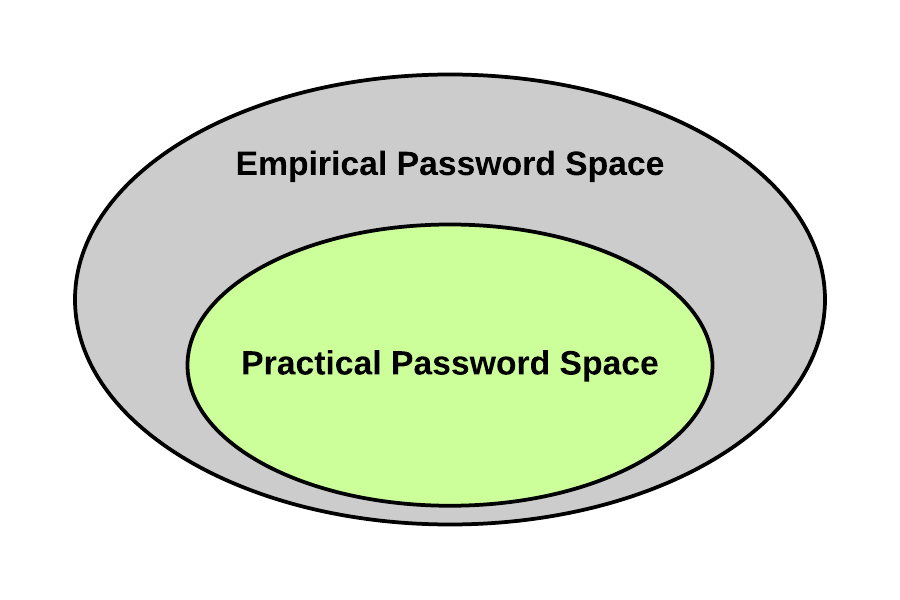
\includegraphics[scale=0.25]{pics/EmpiricalVsPractical.png}
      \caption{Empirical vs. Memorable Password Space}
      \label{fig:memorable}
    \end{figure}

  In a case study of 14.000 Unix passwords, a research group found a 25\% of the passwords were in a group of words forming a dictionary of $3\times10^{6}$ words \cite{UnixPasswords}. This dictionary shows that an attacker can have a relatively high success rate for an attack, despite the fact that there a roughly $2\times10^{14}$ 8-character passwords consisting of digits, and upper case and lower case letters. Due to the limitations of human memory, users often choose passwords that are easier to remember, causing a significant number of user-chosen password to fall into a small dictionary, e.g. practical password space \cite{Tao}. A well-designed dictionary is a tiny subset of the full password space, e.g. theoretical password space, which further can be prioritized according to the likelihood for a password to be chosen. It is, therefore, a commonly stated that the security of a password scheme is related closely to the size of its memorable/practical password space, rather than its theoretical password space. The high success rate of dictionary attack against textual passwords is believed to be strongly related to the recall capabilities of humans and how they choose their passwords, e.g. making meaningful and thus more easily remembered words are selected as passwords.

  One of the first large-scale studies on web password habits was conducted in 2007 by Microsoft research \cite{habits1}. They analyzed web password habits among 544960 Internet users over a period of 3 months. The data was collected from a Windows Live Toolbar, and they observed activities like login frequency. They also gathered information about the users age, the strength of the users passwords, as well as number of unique passwords and its use across different URLs. They observed that a typical user have an average of 7 distinct passwords and that an average of 5 of these passwords was re-used on different web pages. An estimate of the average number of account per user was estimated to be 25 accounts per user, but this would probably be higher since it seven years ago.

  Because of the shortcomings with a text-based authentication, graphical authentication are getting increased attention because it is an alternative to a text-based authentication trying to cope with the memorability and security issues of text-based password. Graphical passwords are using images and visual objects in the authentication instead of text and numeric values. When comparing text against visual objects, the human brain is more capable of remembering images than text. When the human brain is more suited for remembering images, the users might be able to remember more complicated passwords that are not easily guessed. To context where an authentication scheme is used have to be evaluated. Graphical passwords might not fit in all systems, but looks like a good alternative to mobile devices where the user interact with a touch sensitive screen. Typing a long text-based password on a small keyboard on a mobile device is not easy. When using, graphical passwords are easier to interact with on a small mobile screen.


	% Chapter 3 - Litterature Study
	\chapter{Litterature Review}

	{\bf \color{red} Write introduction}

  
  

  


	\section{Graphical Passwords}

% Må få frem hvilke grafiske passord som er laget, samt se på hvilke problemer de løser/ikke løser
% Kommentar fra Lillian: Hva søker man etter når man lager nye passordmekanismer? (entropi, vanskelig å gjette, lett å huske)

  Like text-based passwords schemes, graphical password schemes are also a knowledge-based authentication scheme, e.g. ``something you know'' that are described in the background theory. Since it all started around 1996, there have been many suggestions for graphical password schemes. When a new password scheme are proposed, there are several aspects of password that needs to be considered. A password scheme needs to be secure in terms of entropy, it needs to be hard to guess and it also needs to be easy to use. This section will give a brief introduction to the history of research published on graphical passwords. This is important to know because each scheme is trying to improve different aspects of graphical password, giving us a detailed understanding of todays situation. 

  The idea of graphical passwords was originally described by Greg Blonder in 1996 \cite{Blonder}. The graphical password scheme proposed was requiring the users to tap on a selection of points on a predefined image in order to pass the authentication process. This was just a proposal, and did not further explore the power of graphical passwords, nor analyzed the security aspects of the proposal. 

  In 1999, Jermyn et al. \cite{Jermyn} suggested a new graphical password scheme called ``DAS'' (Draw-a-secret). Draw-A-Secret (DAS) was the first recall-based graphical password scheme proposed. The motivation for the graphical password scheme was that graphical input devices enables the user to decouple the position of inputs from the temporal order in which they occur, and shows that the decoupling can be used to generate passwords that have a larger and more memorable password space. In order to make a more memorable password, the research group argued that the DAS was more secure than text-based passwords because the users were able to remember longer and more complex passwords. After the DAS scheme was published, Dunphy and Yan \cite{BDAS} added an extra background image, called ``BDAS'', in order to encourage their users to make more complex passwords.

  In 2000, Dhamija and Perrig \cite{DejaVu},created a new password scheme called ``Deja Vu''. The password scheme was based on the hash visualization technique \cite{HashVisualization}. The users are asked to select a sequence of images from a random set of images that are generated by a program. They wanted to make a graphical password scheme that solved some of the shortcomings with recall-based authentication like PIN's and text-based passwords. Deja vu should purely rely on recognition rather than recall, and it should be hard to write down and share the password with others. The randomly generated pictures based on the hash visualization technique makes it hard to share the password since the pictures is hard to recreate, but are easy to remember. 

  ``Passfaces'' is a graphical password scheme developed by Real User Corporation that was founded in 2000 \cite{passface}. The authentication procedure allows the users to first select four images that are a visualization on human faces, and the user get authenticated by identifying their four faces. The scheme exploits the advantage that people are good at recognizing people, so when users choose the human faces, they can recognize the characteristics of the faces.

  In 2002, Goldberg et al. \cite{PassDoodle} tried to make a graphical password scheme that combined both text an images called ``PassDoodle''. This is a graphical password combined of handwritten text. Their study concluded that users were able to remember complete doodle images as accurately as text-based passwords.

  In 2004, Davis et al. did a comparison of a light version of the ``PassFace'' and a new graphical password scheme called ``Story'' \cite{Davis}. The Story scheme is making the users choosing images making a story. The background for the scheme was to support their users of remembering their passwords by making a memorable story of images. The story that was made were needed to be recalled in a correct order. To aid memorability, users were instructed to mentally construct a story to connect the everyday images in the set. 

  In 2005 Wiedenbeck and Blonder made a graphical password scheme called ``PassPoints'' \cite{PassPoints} that is an  extension of the Blonder's \cite{Blonder} idea by eliminating the boundaries and allowing arbitrary images to be used. They evaluated their password scheme by testing the scheme on human users. The results showed that PassPoint were a promising scheme with respect to memorability because of the low error rate and low clicking rate. 
  The aim of this study was to get an understanding of how different images affected user performance in authentication with a graphical password scheme. The preliminary result showed suggested that images may support memorability in graphical password schemes. 

  In 2006, a research wanted to address the problem with graphical passwords and the shoulder surfing problem. They called their password scheme ``Convex Hull Click'' (CHC) \cite{Wiedenbeck} that allows the user to prove knowledge of the graphical password in secure and insecure location because they made the scheme in a way that users don't directly click on their password images, making it hard for attackers to do perform shoulder surfing. In CHC the windows shows a list of small icons. In the authentication process, the user needs to recognize some minimum number of their chosen password images, or ``pass-icons'', out of a large number of randomly places icons. This step are presented in a sequence, and if the user responds correctly every time, the user pass the authentication.
  
  In 2007, Tao and Adams \cite{Tao}, created a new proposal for a new graphical password scheme called ``Pass-Go''. The Pass-Go scheme is inspired by the old Chinese game, Go, where users selects intersections on a grid to maker their password. This was one of the first largest user studies on graphical passwords, and was made in order to improve the usability of graphical passwords. They try to emphasize that the usability of a graphical password scheme will increase the memorability of graphical password, causing the password scheme to be more secure.  

  Graphical passwords are also implemented on mobile devices, like the ``Android Unlock Pattern'', that is an mini version of the ``Pass-Go'' deployed on Google Android smartphones. ``PatternLock'' is a similar system that are available for Blackberry. Rather than entering a 4 digit PIN or a text-based password, the user enters a touch-drawn password on a $3\times3$ grid.

  Graphical passwords are still not widely adopted, but there are still new graphical password scheme being proposed. Recently published  graphical password schemes are GeoPass \cite{GeoPass} and Picassopass \cite{PicassoPass}. Geopass is uses a digital map for the authentication phase, where the user chooses a specific location as their password. Picassopass is a graphical password scheme that are presenting a password using a dynamic layered combination of graphical elements. The users can make a story that assists the user in the recognition of the graphical elements.

 \section{Evaluation of Graphical Password Schemes}

  \begin{wrapfigure}{l}{0.35\textwidth}
    \vspace{-20pt}
    \begin{center}
      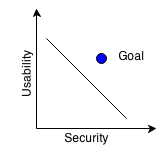
\includegraphics[scale=0.7]{pics/UsabilityVsSecurity.png}
    \end{center}
    \vspace{-20pt}
    \caption{Usability vs. Security}
    \vspace{-10pt}
  \end{wrapfigure}

  Authentication with text-based passwords are a common approach, but it is well known that users often choose weaker passwords because of the limitations of recalling text-based passwords. Graphical passwords came as an alternative solution for overcoming the limitations of text-based passwords, and was inspired by researchers that showed that the graphical memory of humans is particularly well-suited to remember graphical information \cite{DeAngeli}. The problem with many graphical password schemes is that they often promise improved password memorability and thus usability, while at the same time improving the security \cite{Biddle}. This is why it is important to understand both the usability and security aspects when looking at different password schemes in order to understand the trade off between different design choices.

\subsection{Usability and Memorability}

  \todo{Finne forskning som evaluerer grafiske password på usability and memorability}

  An interesting question is what classes of graphical password users find memorable. Based on cognitive studies of visual information, Oorschot and Thorpe \cite{Thorpe1} investigated the memorable password in the graphical password scheme DAS \cite{Jermyn}. They found that the were less or equal to the length of 8 on a 5$\times$5 grid. This results compared to textual passwords may offer greater security against dictionary attacks. 

  If the number of possible pictures in a graphical password scheme is large enough, and the diversity of the of picture based passwords can be captured, it seems reasonable to argue that memorable password space of a graphical password scheme will be higher than text-based password schemes, making graphical passwords offering better resistance to dictionary attacks.
  When the proposal for the graphical password scheme ``Deja Vu'' was proposed, they did a user study that showed that 90\% of all participants succeeded in the authentication tests using Deja Vu while only about 70\% succeeded using pass words and PINS \cite{DejaVu}. This is an example that users tends to have a higher success rate remembering graphical password, rather than text-based passwords. 

  One of the first graphical password schemes, ``DAS'' \cite{Jermyn}, offers a theoretical space that are comparable with text-based passwords, but results from research shows that users tends to draw symmetric images with few pen strokes, and often place their drawings in the center of the grid. The ``BDAS'' scheme \cite{BDAS} tried to avoid this by adding a additional background image, and the results showed that it reduced the amount of symmetry within password images, and supported the users to make longer passwords that were similarly memorable as for the ``DAS''. It remains still a problem that many of the research published on graphical passwords are preformed with a pen and paper approach, raising a question about the validity of the results. One problem may be that many graphical passwords are not implemented, but only a theoretical suggestions. It still remains a lot of research on graphical passwords in their intended environment. 

  Davis \cite{Davis} did a comparison of the memorability between the graphical password scheme ``Face'' (a light version of the ``PassFaces'') and ``Story''. This results reported that users had more difficulty remembering Story password (success rate of 85\%), mostly of the errors was introduced because they had to remember the correct sequence of the images. 

  When looking at usability we can evaluate the graphical layout of a graphical password scheme to see if the visual elements impacts the users choice of passwords. Ullenbeck et al. \cite{Uellenbeck} looked at the Android Unlock patterns and investigated if a change in the graphical layout would impact the security. The Android Patten Lock is made on a 3$\times$3 grid of connected points. Instead they rearranged the points in 4 different positions and analyzed collected data. The results showed that they managed to double the password space by rearranging the points and reduce the biases that are found in the original position of the nodes, but also introduce new ones. One of the rearrangements was a random approach. Unfortunately, this random arrangements of nodes looked like the mathematical ``delta'', so many people recognized the symbol. The random arrangement scored the worst entropy since many of the user chose the same pattern. They did not have several recognizable arrangements, but since people are good at recognizing and memorize patterns, it would not be surprisingly if they would find the same results in other rearrangements that was similar to a user-known symbol.  

  Wiedenbeck et al. \cite{Wiedenbeck1, Wiedenbeck2, Wiedenbeck3} conducted three lab-based user studies of the graphical password scheme ``PassPoint''. The results showed that the users needed an average time of 63 seconds in order to create their password, and an additional average time of 171 seconds in training time in order to remember the password. The login time took an average time of 9 and 19 seconds. This highlights important research of usability and memorability of a graphical password scheme. Some of the factors that makes a password scheme to have hight usability is deiced by average creation time, time to remember the password, as well as time used in the login phase. 

  \todo{Legge til forskning på usability av pass-go}

    
\subsection{Security}

  In knowledge-based authentication, e.g. ``something you know'' we classify attacks into two general categories: guessing and capturing attacks. In a guessing attack the attackers are able to search through the entire password space, or either predict the users passwords patterns in order to avoid searching through the whole passwords space (often referred to as a dictionary attack). This is often associated with the entropy of the password, because the lower the entropy it will be easier to make a successful attack. When talking about capturing attacks, the attackers are able to directly obtain the passwords by observing the authentication process. One of the known capturing attacks on graphical passwords are shoulder surfing because of its graphical visualization.  

  Since a person needs to remember a password, it is normally to choose a password that are connected to you as a person in order to remember the password, causing the password to have bias. A bias can be explained as a prejudice in favor of or against one thing, person, or group compared with another, usually in a way that influence a person choice of action. Since psychological studies have recognized that the human brain have a superior memory for recognizing and recalling visual information, it support the statement that users are able to remember more complex graphical password form a larger password space than a alphanumeric password. Logically the attacker then have to build a bigger and more complex dictionary, thus spend more time to achieve the same success rate as for textual passwords. 

  The graphical password scheme DAS \cite{Jermyn} was evaluating the security of their password scheme. They highlighted that there are many factors that impacts the security of a password scheme, like the statement that the users do not use a uniform distribution of all possible passwords, using Klein's study \cite{UnixPasswords} as a argument. The fact that users do not pick passwords uniformly is not in itself a sufficient statement to make a guessing attack successful. They try to cover the possibility for a attacker making a successful attack by making their scheme complex, and the results showed that the generated passwords was significantly harder to crack in practice than textual passwords. The problem is that they used computer generated passwords that will not show actually password chosen by user. They did not analyze the security of the DAS including human factors and password biases that may could influence the practical password space. 

  There is a lack of analysis on graphical password on users choices in graphical passwords. Davis et al.\cite{Davis} evaluated the security of the ``PassFace'' graphical password scheme. They found that there was a bias that was introduced by the demographics of the users. The users tended to choose faces that they liked and could compare themselves to. The results showed that if you knew the gender and race of a user, you could perform a dictionary attack to guess users passwords. If the gender of a user was known as male, then 10\% of the passwords can be easily guessed on the first or second attempt. Similarly, if the race of a user was known to be Asian and his/her gender is known, then 10\% of the worst passwords can be guessed within the first six attempts. The results indicated that the human passwords was heavily biased, and they stated that the graphical password scheme was insecure. 

  Dirik et al. \cite{Dirik} conducted an experiment by modeling user choice in the graphical password scheme ``PassPoints''. The aim of this study was to test if it was possible to build a dictionary attack based on users choice in clicking points. In this study they predefined two different images with a different level of salient points. The results stated that they could recover 61\% of the users passwords by searching through a smaller password space that was based on a analysis of collected click-points. Normally, the ``PassPoints'' scheme provides user chosen password, but the aim of this study was to investigate if it was possible to predict users password in a dictionary attack. There was a slightly difference in the two images that the researcher picked, where the image with less salient points was stated as insecure. Since the ``PassPoints'' scheme ables the users to pick their own password, the security may relay on the chosen image by the user and not the scheme by it selves. The results from this research can not it selves state that the ``PassPoints'' scheme is insecure, but highlights that it is important to consider the human factors in security because it may influence the total security in a graphical password scheme. 
  The same year another research group published \cite{Thorpe2} results on security of the ``Passpoints'', but using different approaches. They conducted a user studies to test if it was possible to make a offline attack, as well as using a image-processing tool for simulating a offline attack on the same images that were used in the user studies. They provided empirical evidence that popular points, e.g. hot-spots, do exists in images. The results from the most effective attack was generated by harvesting passwords from users to attack other targets. The probability for the guessing attack showed that 36\% of the passwords selected by users could be guessed within $2^{31}$ guesses and 12\% within $2^{16}$ guesses. The results from the offline attack using image-processing were slightly less effective, but they still managed to prove that a offline attack is possible to use on graphical passwords.   

  \todo{Her må jeg ha med flere eksempler på forskning som fokuserer på angrep}

  In one of the first large-scale studies on the Android Pattern Lock \cite{Uellenbeck}, they stated that the entropy of patterns is rather low, and the results from the study indicated that the security offered is less than the security of only thee digits randomly assigned PIN for guessing 20\% of all passwords. In the same research they made a Markov model based on collected passwords from users categorized as offensive and defensive patterns in their user study. The results showed that within 10 guesses they could guess approximately 4\% of pattern in the category defensive patterns and approximately 7\% of the defensive patterns. When increasing the number of guesses to 30 attempts, they managed to guess approximately 9\% of the defensive patterns and approximately 19\% for the offensive patterns. If we look further into the Android Unlock Pattern it have nearly 400.000 possible patterns, and are from a theoretical point of view stronger than a 5-digit randomly assigned PIN. The researchers evaluation of user chosen pattens shows that they only have an estimated entropy slightly lower than a 3-digit randomly assigned PINs. Another interesting result is the memorable password space used, where about 10\% of all users use less than 190 patterns, while less than 300 patterns capture around 50\% of the whole test population. This shows that a empirical password space are not a representative number when quantifying the security of a password, but we should look at the memorable password space, e.g. password that actually are used and memorable. The aim of this study was to close gap of lacking research on the practical password space on graphical passwords. 

  A clever attacker would narrow down the password space and prioritize guesses to pictures that people are likely to choose as a password. The images that are chosen are likely to be the pictures that users are likely to recall. In order to understand how an attacker might take advantage of human password choices, psychological studies on humans visual memory are important to understand. 

\clearpage
\section{Psychology and Human Factors}

  \begin{wrapfigure}{r}{0.35\textwidth}
    \vspace{-20pt}
    \begin{center}
      
\includegraphics[scale=0.35]{pics/dualCoding.png}
    \end{center}
    \vspace{-20pt}
    \caption{Dual-Coding Theory}
    \vspace{-10pt}
  \end{wrapfigure}

  In many years, the field of psychology been a important in order to understand how humans interpret and remember different information. Psychology studies have recognized that the human brain have a superior memory for recognizing and recalling visual information rather than recognizing and recalling verbal or textual information \cite{DeAngeli}. One known theory is the ``dual-coding theory'' \cite{Biddle}, suggesting that verbal and non-verbal memory are processed and represented differently in humans mind. Text are verbal information that is represented symbolically, in contrast to non-verbal information like images that are mentally represented in a way that perceived concepts are assigned to a perceived meaning of what is directly observed. Both verbal and non-verbal information can be used when recalling information. For example, say a person have received stimulus of the concept ``cat'', both the image of a cat as well as the word ``cat''. When the person is asked to recall the concept ``cat'', the person can retrieve the image or the word individually, or both simultaneously. If the word ``cat'' is recalled, the image of the cat is not lost and can still be retrieved at a later point in time. The ability to code a stimulus in two different ways can increase humans ability to remember, in contrast to only code the stimulus in one way. In the background theory there are described three different categories of graphical passwords according to the memory task involved in remembering and entering the password, e.g. recall, recognition and cued-recall. 

  When it comes to humans and visual interpretation, studies supports the idea that people recall symmetric images better than asymmetric images \cite{Attneave, French}. A particular interesting observation is that mirror symmetry carries a special status i the human memory \cite{Wagemans1}. A understanding of psychological studies on humans visual memory can help to build successfully attacks against graphical passwords. If an attacker can successfully use the symmetric properties of graphical password schemes, then the security may be significantly less than if all passwords were equivalent probable. 

  Humans do not only tend to choose symmetric passwords, but do also tend to be influenced by the graphical elements in a password scheme. A study on ``PassFace'' \cite{Davis} showed that there was a high bias in the password selection according to a users gender and race. When they analyzed how each gender choose their password, the most of the male and female participants chose female faces, and and 60-70\% of the user chose a model over a typical female/male. They also looked into the race of the faces, where the results showed that almost all of the participant chose their own race. This research raise the question if it is possible to analyze users choice in passwords based on the demographics of the user.

  A difference in graphical and text-based password schemes is that graphical passwords are able to use images with colors that may influence the users choice in graphical passwords. In a user-study \cite{Thorpe2} on the image-based graphical password scheme ``PassPoints'' managed to see that different images were easier guessed than other images. When analyzing different images and visualizations we can look at studies of gestalt psychology \cite{Wagemans2} that uses the gestalt principles to understand users interpretation of a picture. One of the images that was the easiest to guess in the user-study was a image with cars in different positions in different colors. A possible explanation could be that humans seeks to find pattern that are easily remembered by using the like the principles of grouping, similarities of color, and similarity of size in image analysis.
  \todo{Legge til studier fra psykologi som kan forklare hvordan mennesker ser på sammensetningen av et bilde (cognitive studies)}

  There is a lot of studies on password based on psychology and human factors, but the graphical passwords schemes being analyzed do not look at the background of the users. Humans are different in terms of their demographics, like gender, age and culture in their country. Analysis of people choices of graphical password based on users background have not been looked further into in published research as based on this state of the art research. Since there is a lack of this on graphical password, we will take a look into people choices on text-based passwords based on human properties. 

  %Password habits in subpopulations
  Password habits may be different across different subpopulation in cause of different background or culture. In 2012 Joseph Bonneau released a analysis of 70 million passwords from Yahoo! \cite{Bonneau2}. The data is analyzed in terms of guessing rate by using a dictionary attack. The collected data contained 328 subpopulations. The results showed that there was no ``good'' populations among the collected data, but there was a variation in the population. Demographically, the gender had a small effect in the guessing rate, but it showed that age tended to give effect where password strength increases across different age groups. The analysis also showed that language had a significantly effect on the password strength where Indonesian-speaking users were among the weakest subpopulations, and in contrast the German and Korean-speaking users provided relatively stronger passwords. 

  \todo{Legge til mer forskning}
  

  \section{Graphical Passwords and Mobile Devices}
  %Intro
  Users are not only dependent on remembering passwords across multiple web pages and systems, but do also need to remember passwords for our small mobile devices. The mobile phone have emerged as a good platform for graphical passwords because it is easier to input on touchscreen as a contrast to text-based passwords. Graphical passwords on mobile devices seems as a natural fit, as they often require direct manipulation of visual elements. In todays society we're addicted to our mobile devices in our every day life. Mobile devices are not just a communication tool for calling and texting, but also an important tool for every day tasks like doing our work, reading mail, pay our bills and keeping up with our social life. This trend makes our mobile devices vulnerable in terms of security. To avoid unwanted access, smartphones offers different locking mechanisms. The history of locking mechanisms was often a solution solely to prevent accidental use, while current mobile phones require protection in order to secure the potentially vast amount of private data that we keep on our smartphones. The situation of our rapidly use of mobile phones, as well as it well suited platform for graphical password, makes authentication on mobile devices an interesting field of study.

  When looking at mobile security it essential to be familiar with the magnitude of mobile phone usage. As of 2014, over 90\% of American adults owns a mobile phone, whereas 58\% of American adults owns a smartphone \cite{MobileUseage}. Another 34\% of the users used mostly their phone to go online instead of using other devices such as a desktop or laptop computer. This is numbers from USA, but it still provides insight into the how common mobile phones is today.

  % Awareness about the sensitivity of the data stored mobile phones
  As stated earlier, smartphone user's tends to store sensitive information on their phones, it is therefore important to understand the relationship between the use of security features and users risk perceptions. One of the key security aspects on mobile phones that is important to understand is why people use or not use locking mechanisms on their smartphone. Engelman et al. \cite{Egelman} published a research paper in cooperation with Google on peoples smartphone locking behavior and attitudes towards security of their smartphone data. They observed a strong correlation between use of security features and risk perceptions. They reported that 33\% of the smartphone users were thinking about the locking mechanisms as too much of a hassle, while 26\% of the user's didn't think that someone would care about the information stored on their phone.  Other reported results have covered that the 46.8\% of the participants agreed or fully agreed that unlocking their phone can be annoying, but at the same time 95.5\% of the somewhat or fully agreed that they liked the idea that their phone was protected \cite{habits3}. A study reported that 29\% did not lock their smartphones \cite{MobileUseage}, while another research stated that among 35\% of mobile users don't lock their phone \cite{Bruggen}. The number may vary because of the background and experiences with security , but the number still remains quite high. This highlights that the users wants to be secure, but there might be a trade-off between the time used to unlock the smartphone vs the security risk. 

  % The time used on unlocking the phone
  In terms of security it is interesting to look at the use of mobile devices and look at the locking habits among users on mobile devices. It is known that services that are rapidly used have weaker password because of the overhead the user needs to spend on typing their password. In 2014 a group of researchers published a field study of smartphone (un)locking behavior \cite{habits3}. Some of the problems with smartphone users tends to be their rapidly use of their phone. When the device are rabidly use, it results in a lot of time unlocking their phone between every use. In the study they found that there was a significant overhead in the time used of unlocking their phone, where the users participated in the field study used 2.9\% (9\% in the worst case) of their time unlocking their smartphone. 

  It is stated that a lot of user's use their smartphones to perform tasks that involve use and storage of sensitive data. Smartphones in use today do not require their users to have a locking mechanism on their smartphone. It is well known that users tends to choose to easiest way out and may result in the choice of not having any locking mechanism at all. Based on the result of the overhead in time used on unlocking their phone, a result may be to take the easiest way out by ignoring the vulnerability of not using a locking mechanism at all. It have been discovered that over 40\% of the users only used a basic ``slide-to-unlock'' mechanism on their smartphone, as well as over 16\% didn't use any locking mechanisms at all \cite{habits3}. This highlights a major bad habit among mobile users. What happens if your mobile is stolen? A loss of a mobile phone is not just the cost for replacing the phone, but also a loss of sensitive data. If the phone is found by the wrong persons, the sensitive data on the phone may be lost and used for unintended purposes. A 2012 report from Pew Internet estimated that nearly a third of cell phone users have had their device stolen or lost \cite{StolenLost}. It is interesting to comparing peoples locking behavior towards phones that are stolen or lost. The same report also reported that 12\% of cell owners say that another person have accessed their phone, making the owners feel that their privacy have been exposed to the public.

  Beside loosing a physical device, what consequences are users exposed to? One point of attack is a persons email. If you can grant access to someones email, you probably can get access to a lot more. In a study reported that all of their interview participants had their email account automatically logged in, as well as 31\% of them did not use any locking mechanism at all \cite{Egelman}. The same research group investigated how much information you could gain from getting access to a persons email account. The results showed that both users with or without locking mechanisms found sensitive information in their email account like SSN, Bank Account Number, Email Password and Home Address.

  One of the popular password schemes on smartphones are the Android Unlock pattern. It is a graphical password scheme that have been shown to have biases when the password are user-chosen. A research group did one of the first large-scale user study on the security of the Android Unlock Patterns in order to quantify its security \cite{Uellenbeck}. They analyses the biases introduced in the pattern making process and added changes to the scheme in order to avoid the known biases in the password scheme. The researchers found that there is a high bias in the pattern selection process, e.g. the upper left corner and three-point long straight lines are very typical selection strategies. If the patterns was uniformly chosen, the probability of starting in at any point should be 11\%. The results showed that there was a strong bias of the starting point towards the corners. If the points were uniformly chosen, the probability for all four corners should be 44\%, but the results showed that the probability is close to 75\% in the pen-and-paper study. In contrast to this, the center point, the right, the upper, and the lower center points only get a probability of 14\% based on the results. Other results from the pen-and-paper study found that the average pattern length was 5.63 (with a standard deviation of 1.5). By looking further into the pattern length chosen by users, this is not a surprisingly result because this looks quite familiar with restriction of the Android Pattern Lock that requires the users to make a pattern of at least 4 connected points. As stated earlier, users tends to take a easy way out, making users choose short patterns that are easy to remember and type. Besides the pen-and-paper study, there was also conducted a user study that also showed a high bias towards the upper-left corner that had the bias of 43\% in the user study, and 38\% in the pen-and-paper study. This is supporting the researchers claim that users tends to choose less secure patterns ``in the wild''. 

  The way that the mobile phone is held, the size of the screen may also impact the way that people write their passwords, but this may need further research to answer.

  

	\section{Discussion}

	{\bf \color{red} ** Oppsummere hva jeg har funnet og konkludere med hva som kan forskes videre på ***}

	% Chapter 4 - Design
	\chapter{Results - A Proposed Research Design}
  \label{chapter:researchDesign}

  In this chapter, we will continue with the results from the literature review by looking at a proposal for a research design. The content in this chapter will be a preparatory work for my master thesis that will be conducted in the following spring.

  Section~\ref{sec:hypothesis} is the proposed hypothesis to be used in my master thesis and is a result of the discussion of the literature review in Section~\ref{sec:resultsLiteratureStudy}. Section~\ref{sec:researchstrategy} is a discussion of the possible research strategies to adapt when conducting the research. The research strategy includes a review of the data that looks interesting to look further into based on the proposed hypothesis. Other aspects of the research design like sampling frame, sampling technique, sample size, and response rate is also discussed to provide a complete research design. When selecting a research strategy we need to choose the corresponding data collection method the selected data collection is determined in Section~\ref{sec:researchstrategy} and is further discussed in Section~\ref{sec:datacollection}. When looking at the data collection, this section will further describe the administrative part of the data collection, the questions to be asked, as well as a proposed prototype for collecting the data. The prototype is illustrated in Section~\ref{sec:wireframes}. Along with the wireframes, there is conducted a usability test. Description of the tests, the results, and suggested improvements is described. The prototype will be implemented in the next semester and will not be a deliverable for this project thesis. Section~\ref{sec:ethical} will be an evaluation of the ethical aspects of the research. Unethical research should not be accepted, and the research that is designed must be evaluated and argued to be within ethical guidelines.


  
   

 

  

  %   \subsection{Pattern Lock Functionality}
      
  %     \todo{Beskrive hvordan jeg forholder meg til Funksjonalitet som Android bruker}

  %     When the user first starts using the phone, they are prompted with the choise of using a locking mechanismn on the phone. The functionality of the Android Unlock Pattern are as follow: 
  %       \begin{enumerate}
  %         \item At least four points must be chosen,
  %         \item You cannot visit the same node twice.
  %         \item Only straight lines are allowed, and
  %         \item One cannot jump over point not visited before
  %       \end{enumerate}

    
  %   \subsection{Success Criterias}

  %       \todo{Diskutere hvilke faktorer som er viktige å være obs på i datainnsamlingen}


  % \section{Data Analysis}

  %   \todo{Bestemme hvilken type dataanalyse jeg vil ha. Dette er en følge av hvilke valg jeg har tatt i strategi. Quantitativ eller Qualitativ dataanalyse?}






	\section{Hypothesis} \label{sec:hypothesis}
    
  {\bf $H_{0}$: Human properties have no influence in users choice of graphical passwords} 

  {\bf $H_{1}$: Users choice of graphical passwords are influenced by the human properties of the user}

  The tested hypothesis is referred to as the null hypothesis (abbreviated $H_{0}$). We start with the assumption that the null hypothesis is true; human properties have no influence on users choice of graphical passwords. Along with $H_{0}$ it is stated an alternative hypothesis (abbreviated $H_{1}$). The alternative hypothesis states that users choice in graphical passwords is influenced by the human properties of the user. If the null hypothesis is rejected, we accept the alternative hypothesis.

  The results of this research will have some limitations. {\it First}, the hypotheses do not include all potential human properties. If the results of the statistical test are accepting the alternative hypothesis, the results are not valid for proving a correlation between users choice in graphical passwords and human properties that are not selected in this research. 
  {\it Second}, the hypothesis does neither prove that human choices based on the human properties is valid for all graphical password schemes. The selected graphical password scheme is the Android Unlock Pattern and the decision for choosing this particular scheme is described in the summary of the literature review (Section~\ref{sec:resultsLiteratureStudy}). 
  In the research strategy, there will be a description of the selected human properties (Section~\ref{sec:datarequirements}) that this study find relevant to users choice in graphical patterns.
  
  The results from this study can further be used to evaluate the security of the Android Unlock Pattern. If there is a correlation between users choice in Android Unlock Patterns and the users human properties, it can be used to make dictionary attacks by predicting user's pattern locks. An ability to predict user's choice in locking patterns is a reduction in the scheme's security. It is desired further to suggest improvements of the Android Unlock Pattern scheme and could reduce the predictability of user's choice in locking patterns.

\section{Selection of Research Strategy} \label{sec:researchstrategy}

  This section will provide information about the chosen research strategy.

  A research strategy is the overall approach to answering the main research question. Briony J. Oates \cite{empiriske} presents six different research strategies: survey, design and creation, experiment, case study, action research, and ethnography. This section will not go further in describing the difference between the six strategies, but rather elaborate my choice in research strategy. Out of the six strategies, there is only two of them that are suited as a strategy for this research: survey and experiment. 

  {\it First}, the experiment needs an controlled environment. The data required for the analysis is required to be collected ``worldwide''. It is therefore preferred a research strategy, like a survey, to be able to collect quantitative data without any need for a controlled environment with physical interaction or face-to-face communication.
  {\it Second}, in an experiment, the aim is to study cause and effect relationships when a particular factor is introduced or removed. When looking for correlations between users choice in locking patterns and human properties, there is no such factor added or removed.
  {\it Third}, when analyzing user's choice in graphical passwords, we aim to obtain the same kind of data from a large group of people, in a standardized and systematic way. Later, we want to be able to find patterns in the data using statistics to be able to generalize the results to a larger population. The standardized format can easily extract the collected data without any need for manually work.
  {\it Fourth}, for finding patterns in the collected data, a big amount of data needs to be collected. With a survey, we can use the Internet for distributing a questionnaire for collecting quantitative data. 

  The survey is a good fit for this research along with a questionnaire as the supporting method for collecting data. It is important to understand that there is a difference between a survey and a questionnaire. A survey encompasses all aspects of the research process like design, sampling, data collection, and data analysis. A questionnaire is used as a instrument that is a set of questions to be asked to the participants of the survey.
  
  A limitation of the chosen approach is that it do not support control of the respondents. The questionnaire is distributed over the Internet, and we will not be able to control who will answer the questionnaire. Also, since the data collection is distributed over the Internet, it is not possible for me to judge the accuracy and honesty of people's responses. Despite the limitations, the survey is chosen due to the amount of data needed for the analysis, as well as the lack of time for choosing other approaches, like interviews and other observation techniques. 
  
  In the next section, we will look at the survey in detail. 
  The detailed design of the questionnaire will further be described in Section~\ref{sec:datacollection}.

  \section{Research strategy}

  This section will include important details when using a survey. 

    \subsection{Human Properties} \label{sec:datarequirements}
    
    It is important to analyze what kind of human properties that may impact users choice of lock patterns on mobile devices. We must carefully consider which human properties we want to collect.{\it First}, when a questionnaire is distributed on the Internet there is no way back, and we need to be sure that the chosen questions will provide sufficient and relevant data for answering the hypothesis. {\it Second}, we need to review all human properties and only select a suited number of them. A too long questionnaire may result in a small number of responses because the time needed to complete the questionnaire if all the properties is included. {\it Third}, some of the properties may not have a easy grouping of answers, and may be complex to include in a questionnaire that needs to be answered on a mobile device. If such a property is included, it needs to provide irreplaceable and valuable information for the analysis. The questionnaire should try to avoid time consuming and complex questions if possible. 

    As a result of this review is a list of human properties that this study finds relevant. A narrowed selection of the list will further be included in the data collection (Section ~\ref{sec:datacollection}).  

    \begin{itemize}
      \item {\bf Age:} A group of people within a certain group of age may have different risk awareness. A person with a age between 30-40 and a person with a age below 20 may have different concerns with security. A person in the age between 30-40 may use their phone to perform task with a high security risks like making and job related tasks, while a person with a age below 20 may not have the same security awareness because of the different use of mobile devices.
      \item {\bf Gender:} Psychological studies have reported that males are more likely to take risks than females \cite{Byrnes}. In the literature review there was no reported results found on genders risk awareness in information security, nor peoples choice of patterns based on gender. By analyzing peoples choice of patterns based on users gender might give interesting results. 
      \item {\bf Nationality:} This demographic information is sometimes used in research for graphical passwords. When asking a person about their PIN code, a nationality can be used to find likely numbers to appear because some cultures associates a number to a historical or religious event. In a research on the ``PassFace'', this property was used and proven to be valuable because people tended to choose faces from the same race and nationality. In my research it is uncertain how much this information will help to prove any connection to the choice of patterns. Properties like language preference and reading/writing orientation look more promising in this research.
      \item {\bf Language preference:} By asking the respondent for information about the language preference it can be used to see if the way they write or alphabet they use have any impact on their choice of lock pattern.
      \item{\bf Occupation:} This information is valuable information due to the knowledge level of the respondents. The occupation of the a respondent are simply if the person is a student, employed, not employed or retired.
      \item {\bf Profession:} The profession of a person may say something about a persons knowledge and background. When looking at profession, a person with a profession in IT may be more certain about the security aspects than people in other professions. It may cause bias in the data if people with enough knowledge of security overcompensate their choice of lock pattern because they want to prove their knowledge.  
      \item {\bf Left- or right handed:} An interesting property of humans is the fact that people write with either left or right hand (and sometimes both). This property can influence the way a person are holding the mobile phone, and may impact the way that a person is choosing their pattern. In the literature review it was not found any studies that reported results of people choices in patterns based on the hand used. Published research \cite{Uellenbeck} found that over 40\% of the participants in a study started their Android pattern by starting in the top left corner, but did not record the hand used when making the pattern. My hypothesis is that a left handed person may be using the left hand while interacting with the phone, making the probability for starting in the right upper corner bigger. This have never been tested before and need further research before making a statement. 
      \item {\bf Reading/writing orientation:} In different cultures, there is a difference in the reading and writing orientation. Cultures from Europe and America is normally writing and reading horizontally from left to right, but there are other cultures that do otherwise. Traditionally, Chinese, Japanese, and Korean are writing text vertically in columns from top to bottom, from right to left. Another writing orientation is horizontal from right to left that are used in Arabic cultures. Today, the vertical orientation from top to bottom is often in a horizontal way due to the influence of English and the increased computerized typesetting, but both ways are still in use. There are research that have reported that the writing orientation are affecting the visual attention and memory \cite{Chan}. They found that the reading orientation affected the way a person would memorize objects. They reported that English and Chinese speakers tended to remember an image that appeared in the top, left-hand side of the screen and the Taiwanese speakers tended to remember the images in the upper right-hand side of the screen. The interesting aspect of the reading and writing orientation is to see if people from different cultures are choosing different patterns due to their writing orientation.
      \item {\bf Hand size:} Smartphones today tends to get bigger and bigger in size. An interesting analysis could be done by looking at a users choice of patterns based on size of their hands and size of mobile phone where a patterns is made. By looking at a situation were a person with a small hand and a big mobile device, it may be hard to reach certain areas on the screen by holding a device in one hand, and therefore impact the choice of pattern. 
    \end{itemize}

    \begin{figure}[H]
      \centering
      \subfigure{
        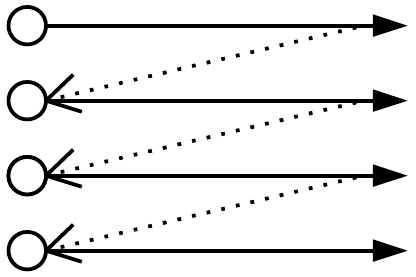
\includegraphics[scale=0.25]{pics/leftright.png}
      }
      \subfigure{
        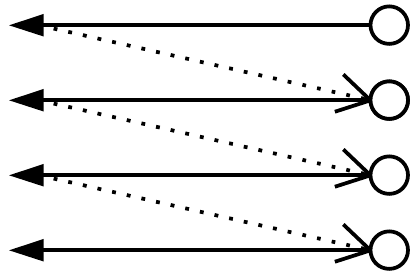
\includegraphics[scale=0.25]{pics/rightleft.png}
      }
      \subfigure{
        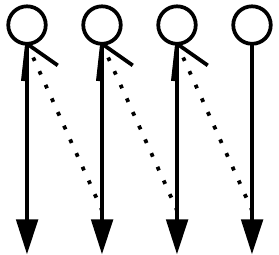
\includegraphics[scale=0.27]{pics/topbottom.png}
      }
      \caption{Writing orientation: 1) Horizontally Left-to right, 2) Horizontally Right-to-left 3) Vertically Right-to-left}
    \end{figure}

    As a result from this review of different human properties, there is need for making a narrowed selection of of the listed properties that looks promising to give any results in the analysis. As stated earlier, the goal of this research is not to prove that all human properties will impact users choice of patters, but make a selection of human properties that this study find promising to look further into. The human properties that will be included in the analysis is the  "reading/writing orientation", "hand size", "Left- or right-handed". Beside the the three main selected properties, I want to collect some demographics and other background information about the users and their mobile devices. This will further be described in Section~\ref{sec:datacollection}. We will now (Subsection~\ref{sec:scenario}) look further into the selected properties in hypothetical scenarios to provide further understanding of the selected properties and possible observations that may occur when analyzing the collected data. 

    \subsection{Sampling Frame and Technique} \label{sec:sampling}
      
      The survey type is categorized as ``non-probability sampling'' and the chosen sample technique is ``self-selection strategy''. This is chosen due to time and cost estimates, and the lack of control of respondents. A Purposive sampling technique would maybe provide a more uniformly collection of people, but it is hard to control respondents when the questionnaire is distributed on the Internet. The self-selection strategy will collect data from any respondents, and will be helpful when there is big population with potential respondents. The self-selection is a useful technique when we are not able to directly contact the potential respondents. When people select themselves for research, it might indicate that they have a strong feeling on the subject, or because they think it will bring them personal benefit or approval. 

      The target population for this research is in general all people with a mobile device. Because of the selected human properties and demographics, it is desirable to divide the target populations into subgroups. The subgroups can be used to control the responses during the data collection in order to provide a wide diversity in the data. 

      \todo{Legge til en liste med subgroups}

      We will now look further into some strategies for collecting data in Subsection~\ref{sec:response} from some of the subgroups that is outside my own network that might be harder get responses from.

    \subsection{Response Rate and Non-responses} \label{sec:response}

      When sending out the questionnaire I have no control over how many that are willing to respond, or how many people from different subgroups I am able to reach. To be able to reach the amount of data needed for a analysis, I need to look for a strategy that may increase the number of responses from the different subgroups. If I suspect that certain types of people in my sample are less willing to respond or harder to reach. I could deliberately include more of that subgroup in my sample so I can assure that I receive the number of respondents that I need. Maybe go face-to-face if a special group of people may be less willing to participate. 

      In this list there will be made a strategy for collecting data from the  different subgroups. {\it First}, some subgroups might be less willing to respond to the questionnaire. {\bf Second}, some of the subgroups might be harder to reach because they are outside of my own network. 

      \begin{itemize}
        \item {\bf People with age of 50 or higher:} People with the age over 50 may not own their own smartphone, or may be hard to reach for other reasons. I need to find networks were there is a high representation of people with a age of 50 or higher. In Norway there is a network called ``Seniorweb''. There is also a magazine called ``vi over 60'' that is a network that is highly represented with people with an age over 60. Both networks are possible to contact if there is a lack of respondents from this subgroup. 
        \item {\bf People with a different field of interest than IT and security:} My own network is overrepresented by people with a profession in IT and security. I need to be able to find other networks to be able to reach out to other people wither other professions. To reach out to people with other professions, it is a possibility to use the network from my family or directly contact a company. The university is a good start because of the high representation of different field of study. 
        \item {\bf People with a reading orientation from right-to-left:} The main reading orientation is from right-to-left, with a exception with some Arabic an Asian nationalities. My network do not include a high sample of people that have a other reading and writing orientation than my own. To reach out to other nationalities I can contact NTNU and ask for help to distribute my questionnaire to countries where NTNU have exchange programs. ``International section'' or other networks like ``ISFiT'' (International Student Festival in Trondheim). 
        \item {\bf People living in a different country than Norway:} I need to get in touch with people from different nationalities in order to get diversity in the collected data. I will contact the International Section at my university to ask them to distribute my questionnaire to the exchange students at my university. I am also having a trip to Minnesota in USA in the following spring, and I will use my time there recruiting people to respond to my questionnaire. During this semester I have been talking to researchers in other countries because of their interest in my research. Hopefully, they can provide help to distribute the questionnaire within their own networks. As stated earlier, ``ISFiT'' is the international student festival in Trondheim. There is people traveling from all around the world to Trondheim. 
        \item {\bf People that are left-handed:} There is a significant higher percentage of people that are right-handed, meaning that there is a possibility for getting more responses from people that are right-handed. Selecting a strategy for this is hard because there is not a known official network for left-handed people. There is a possibility for using groups at Facebook like ``Left-Hander's Club'' or the website called ``Left-handers day''. 
      \end{itemize}

      When analyzing the collected data, I need to find subgroups that have responded and those who have to responded. This will be used to make a discussion of why it lacked responses from a particular subgroup. The reason why this is important is because their non-response might be meaningful in its own right, or their lack of responses may have introduced bias in the data. This part is out of scope for this thesis, but need to be considered in the next phase of this research.
    
    \subsection{Sample Size} \label{sec:samplesize}

      I need to decide how big I want my final sample to be, taking into account my best estimate of the likely non-response rate of participants. When looking at my target population that is very wide. My target population is higher than 1 million, and therefore I would probably would need 1000 respondents or more.

      Because of the lack of control of the diversity of the respondents, there is likely to be some data properties that have a higher representation that others. Therefore it is important to control the data collected during the spring. If it occurs that a subpopulation is overrepresented, it is desired to use the strategy for smoothing the data from Subsection~\ref{sec:response}. The data collected should never be manipulated, and in a situation where there is lack of respondents from a subgroup, the only thing that I can do is to contact networks where there is a higher possibility to reached the subgroup that is underrepresented in the data.

      The total sample size is quite high, but should be manageable. If the total amount of 1000 respondents is not reached, a minimum number of respondents should be accepted at 500. In the analysis it will be hard to make any conclusions if the total number of respondents is too low.  The Internet offers researchers the possibility of accessing many people across the world cheaply and quickly. Not everyone have Internet access, and that need to be considered in the design.

	\section{Data Collection} \label{sec:datacollection}


  \subsection{Form of Administration} \label{sec:formodadministration}

  This questionnaire is a``Self-administered'', meaning that volunteered respondents completes the questionnaire without me being present. This choice is made due time saved, as well as getting enough data. A ``researcher-administrated'' questionnaire would simply be too time consuming and there is a chance that the required amount of data would not be reached. 
    
  When sending the same questionnaire over the Internet, it eliminates the risk of introducing bias by asking the respondents the questions in a different manner, and bias introduced by tone and body language. When collecting passwords, the questionnaire needs to be untraceable back to the respondents due to ethical considerations. A questionnaire over the Internet would make it easier for respondents to share patterns, but it also introduce the problem with the control of the responses and its reliability. The questionnaire needs to be carefully designed in order to reduce possible biases. To get the data in a standardized format, the questionnaire will include closed-question and will therefore generate quantitative data. The asked questions will further be described in the next subsection

  \subsection{Question Content and Responses}\label{sec:questions}

    \subsection*{Pattern selection}
    The pattern selection is divided into 3 different tasks. The reason for doing this is getting more data, as well as setting a pattern into a security setting with different security levels. {\it First}, there is a need for a large scale of data, and by asking the respondents to make three different patterns gives this research more data to analyze. {\it Second}, the pattens now adds a new dimension by categorizing the patterns into three security categories: low, medium, and high. 

      {\bf P1:} {\it Make pattern to protect one of your shopping accounts}

      {\bf P2:} {\it Make a pattern to protect your smartphone}

      {\bf P3:} {\it Make a pattern to protect your banking account}

    \subsection*{Information about the respondents:} 
    This information be used to group respondents in different subgroups to see if there is different choices in patterns in the subgroups. It it also valuable information to collect to see the diversity of the respondents. Some of the interesting human properties selected is the reading orientation. By studying the way humans read we can might use this property to predict users choice in patterns. A theory is that humans would start their pattern in the same direction as their reading orientation. 

      {\bf Q1.1:} {\it How would you categorize the size of your hand?} \\
      The size of the hand can be used to predict likely chosen patterns. Size of the hand is likely to impact the areas the user is able to reach on the mobile screen. This property can be used together with the screen size of the mobile phone in the analysis. 
        \begin{enumerate*}
          \item[ ] {\bf Alternatives:} {\it Small, Medium, Large, XLarge}
        \end{enumerate*}

      {\bf Q1.2:} {\it How would you categorize the screen size of your smartphone?} \\
      As described earlier, the screen size might impact the users choice of patterns. A big screen will maybe introduce areas of the screen that is hard for the user to reach. It is likely that areas that are hard to reach might not be included in the selected pattern.
        \begin{enumerate*}
          \item[ ] {\bf Alternatives:} {\it Small, Medium, or Large}
        \end{enumerate*}

      {\bf Q1.3:} {\it Which hand did you hold you smartphone in when you created the patterns?} \\
      In the review of human properties (Subsection\ref{sec:datarequirements}), it was stated that is was likely that people that was right-handed to start their pattern i the left-upper corner, and that left-handed respondents would start in the right-upper corner. Instead of asking if the respondents are left- or right-handed, I want to ask what hand the respondents are using when interacting with the smartphone. 
        \begin{enumerate*}
          \item[ ] {\bf Alternatives:} {\it Left-hand or Right-hand}
        \end{enumerate*}

      {\bf Q1.4:} {\it What finger did you use when making the patterns?} \\
        \begin{enumerate*}
          \item[ ] {\bf Alternatives:} {\it Thumb or Forefinger}
        \end{enumerate*}

      {\bf Q1.5:} {\it What is you main reading/writing orientation?} \\
      Instead of making assumptions if a nationality have a specific reading orientation, the question is asked directly. A person from Asia do not necessarily write from top-to-bottom.
        \begin{enumerate*}
          \item[ ] {\bf Alternatives:} {\it Left-to-right horizontally, Right-to-left horizontally, or Top-to-bottom Left-to-right}
        \end{enumerate*}

      {\bf Q1.6:} {\it What is your gender?}
        \begin{enumerate*}
          \item[ ] {\bf Alternatives:} {\it Male or Female}
        \end{enumerate*}

      {\bf Q1.7:} {\it What is your age?} \\
      This question will not be pre-divided into specific groups of age. The alternatives in this question will be a open question where the respondents type their specific age. A grouping of the respondents is done when the data is collected.
        \begin{enumerate*}
          \item[ ] {\bf Alternatives:} {\it The specific age of the respondent}
        \end{enumerate*}

      {\bf Q1.8:} {\it What is your nationality?} \\
        \begin{enumerate*}
          \item[ ] {\bf Alternatives:} {\it The selected nationality of the respondent}
        \end{enumerate*}

      {\bf Q1.9:} {\it Have you ever used the Android Unlock Patten?}
      For example, a person with no experience with the Android Unlock Pattern could may introduce bias because the user would not be familiar with its use and functionality. 
        \begin{enumerate*}
          \item[ ] {\bf Alternatives:} {\it Yes or No}
        \end{enumerate*}

      {\bf Q1.10:} {\it Do you use screen lock to protect you smartphone?}
        \begin{enumerate*}
          \item[ ] {\bf Alternatives:} {\it Yes or No}
        \end{enumerate*}

      {\bf Q1.11:} {\it What kind of screen lock do you currently use on your smartphone?} \\
        \begin{enumerate*}
          \item[ ] {\bf Alternatives:} {\it Unlock Pattern, Fingerprint, PIN, Slide-to-Unlock, Other}
        \end{enumerate*}

      {\bf Q1.12:} {\it Is you mobile operating system ``detected OS''?} \\
      The reason for asking this question is to be able to check if the device used to answer the questionnaire provides the pattern lock security mechanism. 
        \begin{enumerate*}
          \item[ ] {\bf Alternatives:} {\it Android, iOS, Windows, or Other}
        \end{enumerate*}

      {\bf Q1.13:} {\it Do you work with IT and/or security full time or studied IT and/or security?} \\
      To ask the respondents about their profession is not easy. {\it First}, the list of potential professions is a long list. {\it Second}, it might take a lot of time for the user to find a suitable alternative that describes their profession. I want to use this question to see if people with a profession in IT and Security introduce bias in the data. People with a profession in IT or security may try to overcompensate to prove their knowledge, or they will make more complex patterns than people with a other profession. The list of statements will ask if the respondents have worked with or studies IT or security. 
        \begin{enumerate*}
          \item[ ] {\bf Alternatives:} {\it Yes or No}
        \end{enumerate*}

  \clearpage
  \subsection{Layout and Structure}\label{sec:layout}

    Before the questionnaire starts there is given some information about the research, the use of the collected data, and privacy concerns. After the information, the respondent will be given the possibility to practice before entering the patterns. This is optional, and is added for users that is not familiar with the Android Unlock Pattern.

    After the training, the respondents will be asked to make a pattern for three different categories of security risks. It is a concern that respondents could make patterns that is done quickly without any thoughts. When asking a person to make a ``complex pattern'', people tend to overcompensate and choose rather complicated passwords. This behavior is well known in psychology as ``priming''. By overcompensating and choosing rater more complicated patterns than probably would appear ``in the wild'' would introduce bias in the data because the overcompensated password is not representative. By asking people to make three different patterns, we get a overview of the complexity without directly asking the users to make a password that is hard to guess.

    After the patterns is entered, the background and demographics of the users will be asked for. There is a thought behind the ordering of the different parts of the questionnaire. {\it First}, people might stop before finishing the questionnaire, and is therefore desired to collect the patterns first. {\it Second}, the additional data collected might impact the users choice in patterns. For example, when asking a person about their hand size, or the size of the screen, the respondent might be aware that this properties will be impacting their patterns. A such observation form the user could introduce bias in the data.

    This is will be the structure of the questionnaire:

    \begin{enumerate}
      \item {\bf Introduction}
      \item {\bf Pattern training}
      \item {\bf Selection of Pattens}
      \item {\bf Background and Demographics}
    \end{enumerate}

  \subsection{Validity and Reliability}\label{sec:validityandreliability}

    {\bf Content validity}

    {\bf Construct validity}

    {\bf Reliability}

  

    %Forstår de hva som skal svares på? Ville de svart på denne undersøkelsen? Er etiske aspekter brutt? Vil det ta for lang tid?

 

  

  

% Bør si noe om vanskeligheten med å samle inn password og forskjellen på å samle inn lekasje of faktiske passord.
% Hva bruker man mobilen til? Bank, facebook, mail, jobb, etc? Kan man se en sammenheng mellom passord og bruk av mobil. 
% Lage passord for forskjellige risikokategorier.


	\section{Prototype - System for Data Collection}
\label{sec:wireframes}

  This section will provide a proposed system for data collection. First we will look at a framework for evaluating the usability of the system for data collection in Section~\ref{sec:usability}. The design choices and the wireframes for the system are described and illustrated in Section~\ref{sec:designChoices}.

  \subsection{Usability} \label{sec:usability}

  When creating a system it is important to evaluate its usability. This section will provide a framework to include when designing the a prototype for data collection. The prototype is further the described and illustrated in the next section.

  Usability is defined as ``the extent to which a product can be used by specified users to achieve specified goals with effectiveness, efficiency and satisfaction in a specified context of use'' \cite{ISO9241}. Figure~\ref{fig:usability} is showing how we are going to measure the usability of the prototype created for data collection.

  The first level contains the usability measures effectiveness, efficiency, and satisfaction. The first usability measure, {\it efficiency}, is defined as ``resources expended in relation to the accuracy and completeness with which users achieve goals'' and is measured at the usability metric time on task. The second usability measure, {\it effectiveness}, is defined as ``the accuracy and completeness with which users achieve specified goals'' and is measured by the usability metrics number of errors and completion rate. The last usability measure, {\it satisfaction}, is defined as ``freedom from discomfort and positive attitudes towards the use of the product. '' and is measured by the usability metric of subjective satisfaction.

  \begin{figure}[H]
    \centering
    
\includegraphics[scale=0.25]{pics/usability.png}
    \caption[ISO9241 - Usability]{ISO9241 - Usability \cite{ISO9241}}
    \label{fig:usability}
  \end{figure}

  The prototype that is being evaluated is a prototype for data collection, e.g., the system. A user is defined as ``the persons who interact with the product'' and is the respondents that answer the survey through the system. The goal of the system is to collect patterns and information about the users. The task that the respondents needs to perform is to provide their answers to the questions asked in the questionnaire (Section~\ref{sec:questions}). The product, for which usability is to be evaluated, is the prototype for the software being implemented on mobile devices.  

  \subsection{Design Choices} \label{sec:designChoices}
    
  This section will be a proposal for how we can build a system for data collection. The system is a prototype of the questionnaire, and will be created as a web application that will be easy to distribute over the Internet. This is only a proposal for a system, and the final system will be implemented next semester. During this project, I have spent much time designing the look and feel of the system, as well as the structure and flow. The final system will only be running on a smartphone.

  When designing a system for a mobile device, there is many usability requirements that must be considered (Figure~\ref{fig:usability}). {\it First}, the system must be efficient to use. When interacting with a small screen, I need to consider how the respondent can complete the questionnaire as fast as possible. The number of questions is quite high, therefore, we need to establish a flow that supports the user to complete the questionnaire quickly. It is not desired to get in a situation where many of the respondents quit before finishing the questionnaire because it takes too long time. {\it Second}, the system need to be effective in terms of the respondent's completion rate, avoiding too many errors. When considering the effectiveness of the systems, the system needs to support the respondents to be able to complete the questionnaire. {\it Third}, when using the system, the respondents need to get a positive attitude towards using the system. This usability requirement is often used to design systems that people want to use. For this system, it may not be a system that people find fun to use, but maybe I am able to design it in a way that people find it interesting. It should also be considered that the respondents feel confident while using the system. The system are collecting patterns created by the respondent, making the system be considered as trustworthy in order to reach a subjective satisfaction from the respondents.

  When designing the system, the first issue was to design the response alternatives and how the respondents efficiently select their answer. For illustrating the answers, I picked out icons that I believe have a universal semantic meaning. By universal semantic meaning, I am talking about icons that people of different ages and different nationalities are familiar with. To illustrate one example, I used an image of a girl and a boy that is usually used on for example toilets (Figure~\ref{fig:boygirl}). When the user is asked for their gender, the two images are visualized as the possible alternatives instead of using text. Using too much text can take too much time to interpret, as well as it might keep the respondent attention throughout the whole questionnaire by using visual alternatives. I also believe that using universal icons support respondents that are not fluent in English to be able to answer the questionnaire.

  \begin{figure}[H]
    \centering
    \subfigure[Male]{
      
\includegraphics[scale=0.5]{pics/male3.png}
    }
    \subfigure[Female]{
      
\includegraphics[scale=0.5]{pics/female3.png}
    }
    \caption{Icons used for illustrate the gender alternatives}
    \label{fig:boygirl}
  \end{figure}

  Since this system only is supposed to be answered by a mobile device, the only input is coming from the touch screen. When the alternatives for each question are illustrated with icons, it is very easy for the respondents to select their answers by clicking on the icon. This helps the users to choose their answers quickly. Other aspects are the error rate and completion rate when looking at the usability measure effectiveness. The icons are easy to interact with from a touch screen. Other alternatives for the respondents to select their answer could be a list of textual alternatives. Such icons are called radio buttons and are often small. This can cause a situation where a person selects an answer that was not intended. I believe that using big icons can reduce the error rate, as well as raise the completion rate. This might also increase the subjective satisfaction because it may avoid an annoying situation where it takes too long time to interpret the alternatives, as well as avoid misplaced answers.

  When answering a questionnaire it is important to indicate the progress, e.g. how far the respondent is from completion. This will support the satisfaction of the user. The progress can be illustrated with a progress bar or percentage/number of completed answers. If there is no indication of the progress, there is not added any ``award'' for answering each question. When the respondents can see the progress for each completed answer, they may feel that they were getting an award and therefore feeling satisfied.

  The flow and structure are also an important aspect of usability. As stated, the respondents should be able to complete the questionnaire as fast as possible. When designing the wireframes for the prototype, it is hard to use flow elements that often is used on mobile devices. Such elements are animation and automatic progress. I have chosen to use arrows to support the flow and progress in the prototype because other features is hard to illustrate on paper. The flow is, therefore, added to further discussion in Chapter~\ref{chap:FutureWork}.

  The next section will include the wireframes for the prototype. Figure~\ref{fig:navigation} is four of the icons used in the wireframes for the navigation and progress. Figure~\ref{fig:left} and Figure~\ref{fig:right} is the navigation elements used for progressing trough the system. Figure~\ref{fig:help} is an icon used if the respondent does not understand the question, and will provide extended information. Figure~\ref{fig:progress} is the progress bar indicating the progress in the questionnaire. 

  \begin{figure}[H]
    \centering
    \subfigure[Navigate left]{
      
\includegraphics[scale=1]{pics/leftarrow5.png}
      \label{fig:left}
    }
    \subfigure[Help]{
      
\includegraphics[scale=0.16]{pics/question48.png}
      \label{fig:help}
    }
    \subfigure[Navigate right]{
      
\includegraphics[scale=1]{pics/rightarrow6.png}
      \label{fig:right}
    }
    \subfigure[Progress]{
      
\includegraphics[scale=1.15]{pics/progress.png}
      \label{fig:progress}
    }
    \caption{Navigation elements}
    \label{fig:navigation}
  \end{figure}

  \subsection{Wireframing - Designing the Prototype}

  The prototype is created with a method called wireframing. A wireframe is low-fidelity prototype design that is sketchy and incomplete. Wireframes are easily constructed at a low cost and is made to avoid design issues when implementing the final system. The wireframes are the first proposal for the data collection system and will be used to test broad concepts of the prototype before the implementation.

  The wireframes in the next section are at version 3 and have been through several reviews. First, I contacted created the first version by mocking up a design. {\it Second}, I contacted an assistant professor, Ole Andreas Alsos, from Department of Computer and Information Science at my university. He also teaching in a course named ``Prototyping Interactive Media'' (TDT4262). I scheduled a meeting with Ole Andreas to get feedback on the first version of the prototype. After the meeting I got much feedback on how to ask questions, as well as feedback on the overall design. This led to the version 2 of the prototype.

  In December 8-10, my co-supervisor, Per Thorsheim, arranged a conference called ``PasswordsCon'' \cite{conference} at my university. At the conference, there were participants from all over the world; all with the same interest in passwords. For me, this was an excellent opportunity for me to talk to researchers and other people with an interest in passwords. Here I met one of the researchers that published the first large-scale user study on the Android Unlock Patten, Markus Dürmuth \cite{Uellenbeck}. I also met a researcher from Cambridge University, Jeunese Payne, that interested in passwords and psychology. Her main field of study is psychology, but she recently works on a project called ``Pico'' at Cambridge University that investigate a new authentication scheme. I sat down with both Markus and Jeunese, and explained my research and the selected research design that is described in this chapter. They both provided feedback on the wireframes and the overall research. At the same conference, I also presented this project thesis \cite{presentation}. The conference was an important event for this research as I got many responses from researchers that were interested in the work I am doing in my master thesis. I got much motivation, as well as retrieved a bigger network of password interested people from all over the world. This will be an important network to have when I am going to collect the data in the next semester.

  At the end of the conference, I gathered the feedback that resulted in version 3 of the wireframes. The final version is described in detail in the next section.

  \subsection{Wireframes} \label{sec:thewireframes}

  This section includes a description of the prototype for data collection illustrated in wireframes.   

    \begin{wrapfigure}{l}{0.35\textwidth}
      \centering
      \vspace{-5pt}
      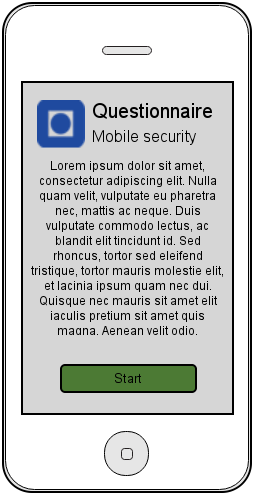
\includegraphics[scale=0.40]{screens/v3/mobile/mobile1-1.png}
      \caption{Introduction screen}
      \label{fig:wireframe1}
    \end{wrapfigure}

  Figure~\ref{fig:wireframe1} is the first screen that the respondents meet when they access the questionnaire. This includes a description of the research, information about the questionnaire, and privacy concerns for the respondent. This is the first part that the respondents meet, so it is important that the defendant feel confident. The contact information provides a creditability to the questionnaire, so the respondents can feel save that information is handled correctly accordingly to the information that is given. It also allows the respondents to ask questions if they have any questions or want to Google the researcher responsible for questionnaire. A questionnaire asking for personal information might seem scary for some respondents, it is then comforting to be able to see who this person is.

  When the respondents are decided to participate, they press start and is transferred to the screen in Figure~\ref{fig:wireframe2}. This screen is providing information about the Android Unlock Patten, so they can know how to type the pattern. If the respondents have not tried the unlock pattern before, they will get the choice to try the scheme before entering their pattern. For experienced users, they can skip the training for saving time. Figure~\ref{fig:wireframe3} shows the training mode. The registered patterns are collected to be able to compare the pattern in the training mode, as well as the selected patterns. Figure~\ref{fig:wireframe4} is the start screen for the pattern creation. The respondents are asked to make three patterns, one for a shopping account, one pattern for their smartphone, and one pattern for their banking account.

    \begin{figure}[H]
      \subfigure[Introduction to Android Lock Pattern]{
        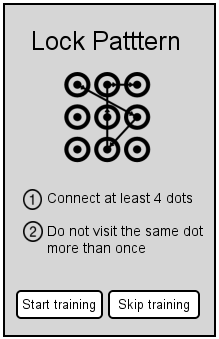
\includegraphics[scale=0.48]{screens/v3/plain/plain1-2.png}
        \label{fig:wireframe2}
      }
      \subfigure[Training mode]{ 
        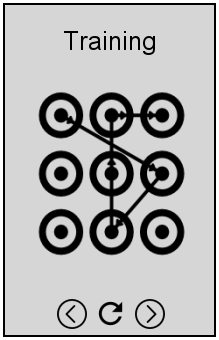
\includegraphics[scale=0.48]{screens/v3/plain/plain1-3.png}
        \label{fig:wireframe3}
      }
      \subfigure[Introduction to pattern creation]{
        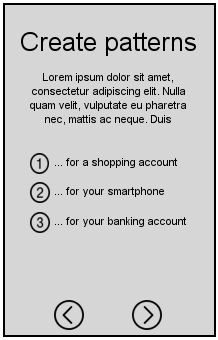
\includegraphics[scale=0.48]{screens/v3/plain/plain1-4.png}
        \label{fig:wireframe4}
      }
    \end{figure}

  The pattern creation is showed in Figure~\ref{fig:wireframe5}, Figure~\ref{fig:wireframe6}, and Figure~\ref{fig:wireframe7}. For different users, the order of the different pattern will occur in a different order using the Latin Square method that was described in Section~\ref{sec:layout}.

    \begin{figure}[H]
      \subfigure[Creation of pattern 1]{
        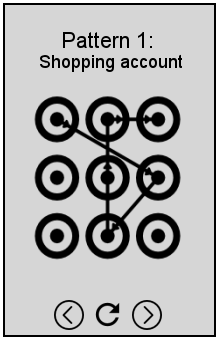
\includegraphics[scale=0.48]{screens/v3/plain/plain1-5.png}
        \label{fig:wireframe5}
      }
      \subfigure[Creation of pattern 2]{
        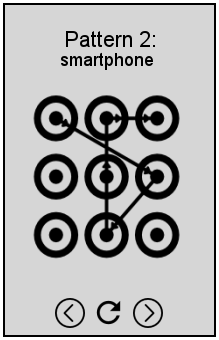
\includegraphics[scale=0.48]{screens/v3/plain/plain1-6.png}
        \label{fig:wireframe6}
      }
      \subfigure[Creation of pattern 3]{
        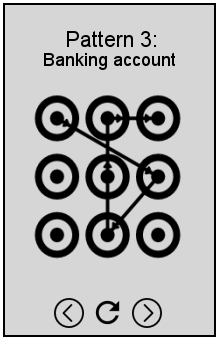
\includegraphics[scale=0.48]{screens/v3/plain/plain1-7.png}
        \label{fig:wireframe7}
      }
    \end{figure}

  The first part have focused on the pattern creation because it is the most crucial information needed. After the pattern creation, the questionnaire will now ask the respondents about demographic, experience and use of lock screens and some information about the device used to answer the questionnaire. All of these questions is found in Table~\ref{tab:questions}, and most of the human properties is found in the analysis of human properties in Section~\ref{sec:datarequirements}.

  Figure~\ref{fig:wireframe8} is asking about the respondent's hand size. The answers from this question will be subjective, but there is not any other way this can be asked. Asking people to measure the actual size would be preferable but would require too much time for the respondents. They also might not have any instruments available to measure their precise length. Figure~\ref{fig:wireframe9} is asking the respondents about their screen size. This will also be subjective. In order to be able to get the correct size, there will be used JavaScript to detect the actual size of the screen in (illustrated in Listing~\ref{list:screen}). Why add a question that is possible to detect automatically? It is not desired to collect data that is not explicitly asked.

  \medskip
  \begin{lstlisting}[caption=Detecting screen size in JavaScript, label=list:screen]
    var height = window.screen.availHeight;
    var width = window.screen.availWidth;
  \end{lstlisting}

  In Figure~\ref{fig:wireframe10} it is asked for the hand used when the respondent answered the questionnaire. This can be used when predicting the likely initial starting point that was discussed in Section~\ref{sec:datarequirements}

    \begin{figure}[H]
    \ContinuedFloat
      \subfigure[Q1: Hand size]{
        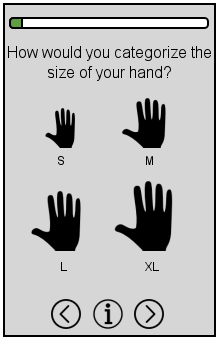
\includegraphics[scale=0.48]{screens/v3/plain/plain2-1.png}
        \label{fig:wireframe8}
      }
      \subfigure[Q2: Screen size]{
        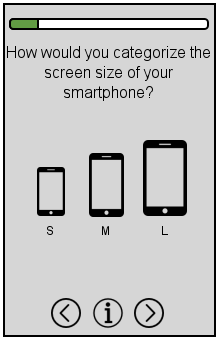
\includegraphics[scale=0.48]{screens/v3/plain/plain2-2.png}
        \label{fig:wireframe9}
      }
      \subfigure[Q3: Handedness]{
        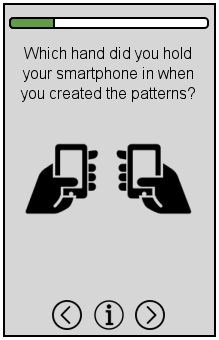
\includegraphics[scale=0.48]{screens/v3/plain/plain2-3.png}
        \label{fig:wireframe10}
      }
    \end{figure}

    When the respondent is using either left- or right-hand, it is crucial to know the finger used (Figure~\ref{fig:wireframe11}). If the respondent is using their thumb, it is likely that they held the smartphone in one hand. If the forefinger is used, it is likely that the respondent used the forefinger. My hypothesis is that this is necessary information to collect because the finger used is deciding which part of the screen they can reach. In the next wireframe the respondent is asked about their reading direction (Figure~\ref{fig:wireframe12}). The most common reading direction in most countries is from left to right. People using Arabic for reading and writing usually have the right-to-left direction. Some countries in Asia (Japan, Korea, China, and Taiwan) is reading and writing from top-to-bottom, left-to-right. 
    The next information is about the user's gender, and is illustrated in Figure~\ref{fig:wireframe13}.

    \begin{figure}[H]
    \ContinuedFloat
      \subfigure[Q4: Finger used in pattern creation]{
        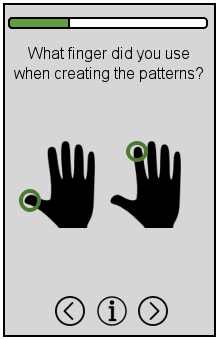
\includegraphics[scale=0.48]{screens/v3/plain/plain2-4.png}
        \label{fig:wireframe11}
      }
      \subfigure[Q5: Reading/Writing orientation]{
        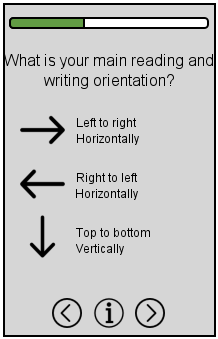
\includegraphics[scale=0.48]{screens/v3/plain/plain2-5.png}
        \label{fig:wireframe12}
      }
      \subfigure[Q6: Gender]{
        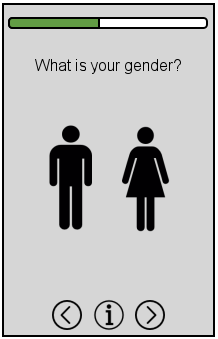
\includegraphics[scale=0.48]{screens/v3/plain/plain2-6.png}
        \label{fig:wireframe13}
      }
    \end{figure}

    When collecting demographics, it is important to know the age of the respondents. It is not known if it will give any results that can be shown to be statistically significant, but it is desired to be able to have a diversity in the age of the respondents. There might be some difference in the risk awareness, or the experience with mobile phones. The age is not grouped into different interval because it is hard to predict reasonable age interval of the sample (Figure~\ref{fig:wireframe14}). The nationality is important to have so it is possible to see how the data is represented on the map. When making statistical tests, it is important to be able to reason about its representation worldwide, or if the results only statistical significant for some part of the world. It is desired to collect data from different nationalities. The respondents selects their nationality from a list. The list might be quite long. To make it easier for the respondents to answer it is possible to map their browser language to their nationality and put them on top of the list. Many respondents might use English as their preferred browser language, then it is not very easy to list specific nationalities on the top of the list. The JavaScript code is illustrated in Listing~\ref{list:language} and the wireframe is illustrated in Figure~\ref{fig:wireframe15}. 

    \medskip
    \begin{lstlisting}[caption=Detecting browser language, label=list:language]
      var browser_language;
      if (navigator.userLanguage) // IE
        browser_language = navigator.userLanguage;
      else if (navigator.language) // FF, Chrome, Safari, Opera
        browser_langauge = navigator.language;
    \end{lstlisting}

    The next wireframe there is a question about whether they have used the Android Unlock Pattern or not (Figure~\ref{fig:wireframe16}). This information can be used to compare respondents that have used the scheme before and those who have not. 

    \begin{figure}[H]
      \ContinuedFloat
      \subfigure[Q7: Age]{
        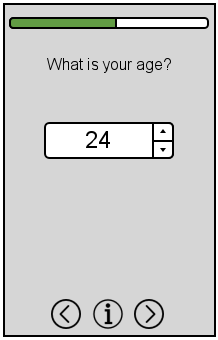
\includegraphics[scale=0.48]{screens/v3/plain/plain2-7.png}
        \label{fig:wireframe14}
      }
      \subfigure[Q8: Nationality]{
        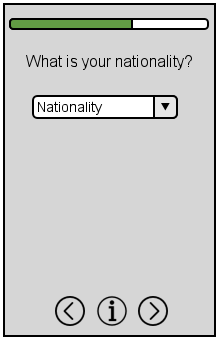
\includegraphics[scale=0.48]{screens/v3/plain/plain2-8.png}
        \label{fig:wireframe15}
      }
      \subfigure[Q9: Android Unlock Pattern experience]{
        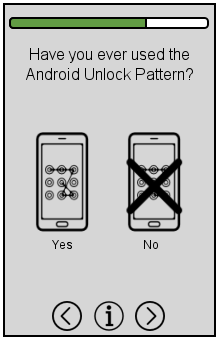
\includegraphics[scale=0.48]{screens/v3/plain/plain2-9.png}
        \label{fig:wireframe16}
      }
    \end{figure}

    Figure~\ref{fig:wireframe17} is asking if the respondents use a screen lock, and if they do, they are redirected to Figure~\ref{fig:wireframe18}. If not, they are directly directed to Figure~\ref{fig:wireframe19}. Figure~\ref{fig:wireframe19} is asking about the mobile Operating System (abbreviated OS) on the mobile used for answering the questionnaire. This is a tricky question to ask because there might be many people that don't know what an operating system is. There are different ways to collect the operating system of the mobile used:

      \begin{enumerate}
        \item You can detect the OS without asking.
        \item You can explicitly ask for the mobile OS and show different icons associated to the mobile operating system (like the apple for iOS and the Droid for Android). 
        \item Combine detection and asking. 
      \end{enumerate}

    The first alternative is not an appropriate way to collect data because I do not want to gather information that the respondents do not know that is collected. The second option is to illustrate the different icons associated with the different mobile operating system. The problem is that the respondent might not know what their mobile operating system is, or they simply don't know what an operating system is. The last option is to detect the mobile OS and then ask the respondent if the detected mobile OS is the mobile OS on their smartphone. It is added an option to answer ``I don't know'' in the case if the respondents feel uncertain. The question is formulated as a generic question: ``is you mobile operating system `detected system' ''. It looks like all participants gets the same question, and the respondents do not get the feeling that the questionnaire is doing something they do not have control over. If the respondent is using an iPhone, the mobile OS can be detected by using JavaScript as described in Listing~\ref{list:mobileOS}.

    \clearpage
    \medskip
    \begin{lstlisting}[caption=Detecting mobile OS, label=list:mobileOS]
      var mobileOS;
      if (navigator.userAgent.match(/iPhone/i)){
        mobileOS = 'iOS';
      }
    \end{lstlisting}

    \begin{figure}[H]
      \ContinuedFloat
      \subfigure[Q10: Screen lock usage]{
        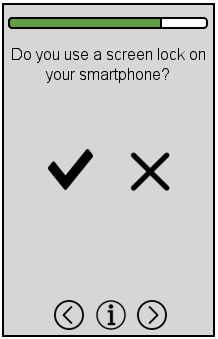
\includegraphics[scale=0.48]{screens/v3/plain/plain2-10.png}
        \label{fig:wireframe17}
      }
      \subfigure[Q11: Selected screen lock]{
        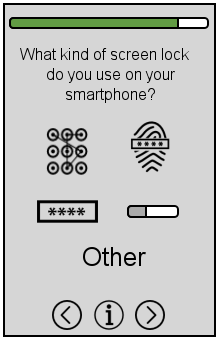
\includegraphics[scale=0.48]{screens/v3/plain/plain2-11.png}
        \label{fig:wireframe18}
      }
       \subfigure[Q12: Mobile OS]{
        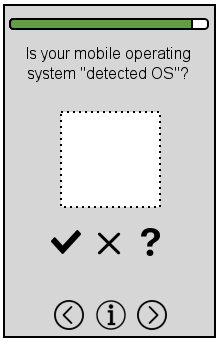
\includegraphics[scale=0.48]{screens/v3/plain/plain2-12.png}
        \label{fig:wireframe19}
      }
    \end{figure}

    The last question is about the respondents experience with IT and security (Figure~\ref{fig:wireframe20}). This question is asked because it is desired to see if people with experience with IT and Security makes different patterns than other respondents. If there is a statistically significant difference, it might introduce bias because they do not represent the whole population. Because of their experience with IT and Security, they might create patterns that are harder to guess. It is also known that people with an interest in security might have a higher interest in participating. The last wireframe (Figure~\ref{fig:wireframe21}) is just a message showing my gratitude to the respondent for using their time to helping by answering the questionnaire. It is here important to provide the same contact information if the respondents have any questions or interest in the study. There might be some respondents that are interested in the results and want to know where they can get the results. 

    \begin{figure}[H]
      \centering
      \ContinuedFloat
      \subfigure[Q13: Experience with IT and security]{
        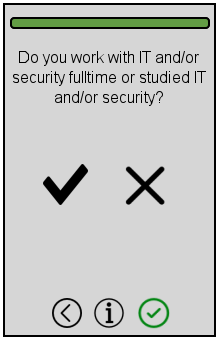
\includegraphics[scale=0.48]{screens/v3/plain/plain2-13.png}
        \label{fig:wireframe20}
      }
      \subfigure[Questionnaire completed]{
        
\includegraphics[scale=0.48]{screens/v3/plain/plain2-14.png}
        \label{fig:wireframe21}
      }
      \caption{Wireframes}
      \label{fig:wireframes}
    \end{figure}



  \subsection{Usability Test}\label{sec:pretest}
  Before implementing the system, I need to perform a usability test on the proposed prototype. {\it First}, I need to figure out if the respondents understand the questions stated in the questionnaire. This can cause bias in the data if the questions asked are ambiguous. {\it Second}, the time needed for completion of the questionnaire can not be too long. If the questionnaire takes too long to complete, there is less likely that people want to spend their time completing the questionnaire. At the same time, there is required a lot of data to be able to make see patterns in the data. Therefore, it needs to be a balance between questions and data collected and time of completion.

  A pen and paper test will be conducted to check whether the wording of the questions as well as getting feedback of the amount of information asked. It is also interesting to ask questions about the ethical aspects of the data collection. If some of the test persons feels that their privacy is leaked by answering the questionnaire, the questions might need to be reevaluated.

  In this report, there will be conducted two usability tests based on using the wireframes from Section~\ref{sec:thewireframes}. We want to measure the usability of the system in terms of efficiency (time on task), effectiveness (number of errors and completion rate), and satisfaction. When conducting the test with printing the wireframes on paper, it is not easy to measure the time used. The time used will not be accurate because there might be a dialog between me and the participants. It will be observed how easily they complete the task, and afterward ask if they felt that the questionnaire took too long of a time to complete. The first test will be a complete run through all wireframes. The second test is only testing the icons used in the wireframes.

  \subsubsection*{Setup}

  For testing the usability of the system, it was conducted two different tests. In both tests, I was acting as the mobile phone, and the participants interacted with the prototype as it was a real smartphone. Whenever they selected an action, I simulated what the system should do.
  Before the test started, it was given some information about the research.  
  
  Test 1 was testing the overall usability by measuring the efficiency, effectiveness, and satisfaction (Figure~\ref{fig:usability}) of the prototype. The corresponding usability measures used was time on task, number of errors and completion rate, and subjective satisfaction. Figure~\ref{fig:test1} is showing some of the wireframes printed on paper that was used during the test. 

    \begin{figure}[H]
      \centering
      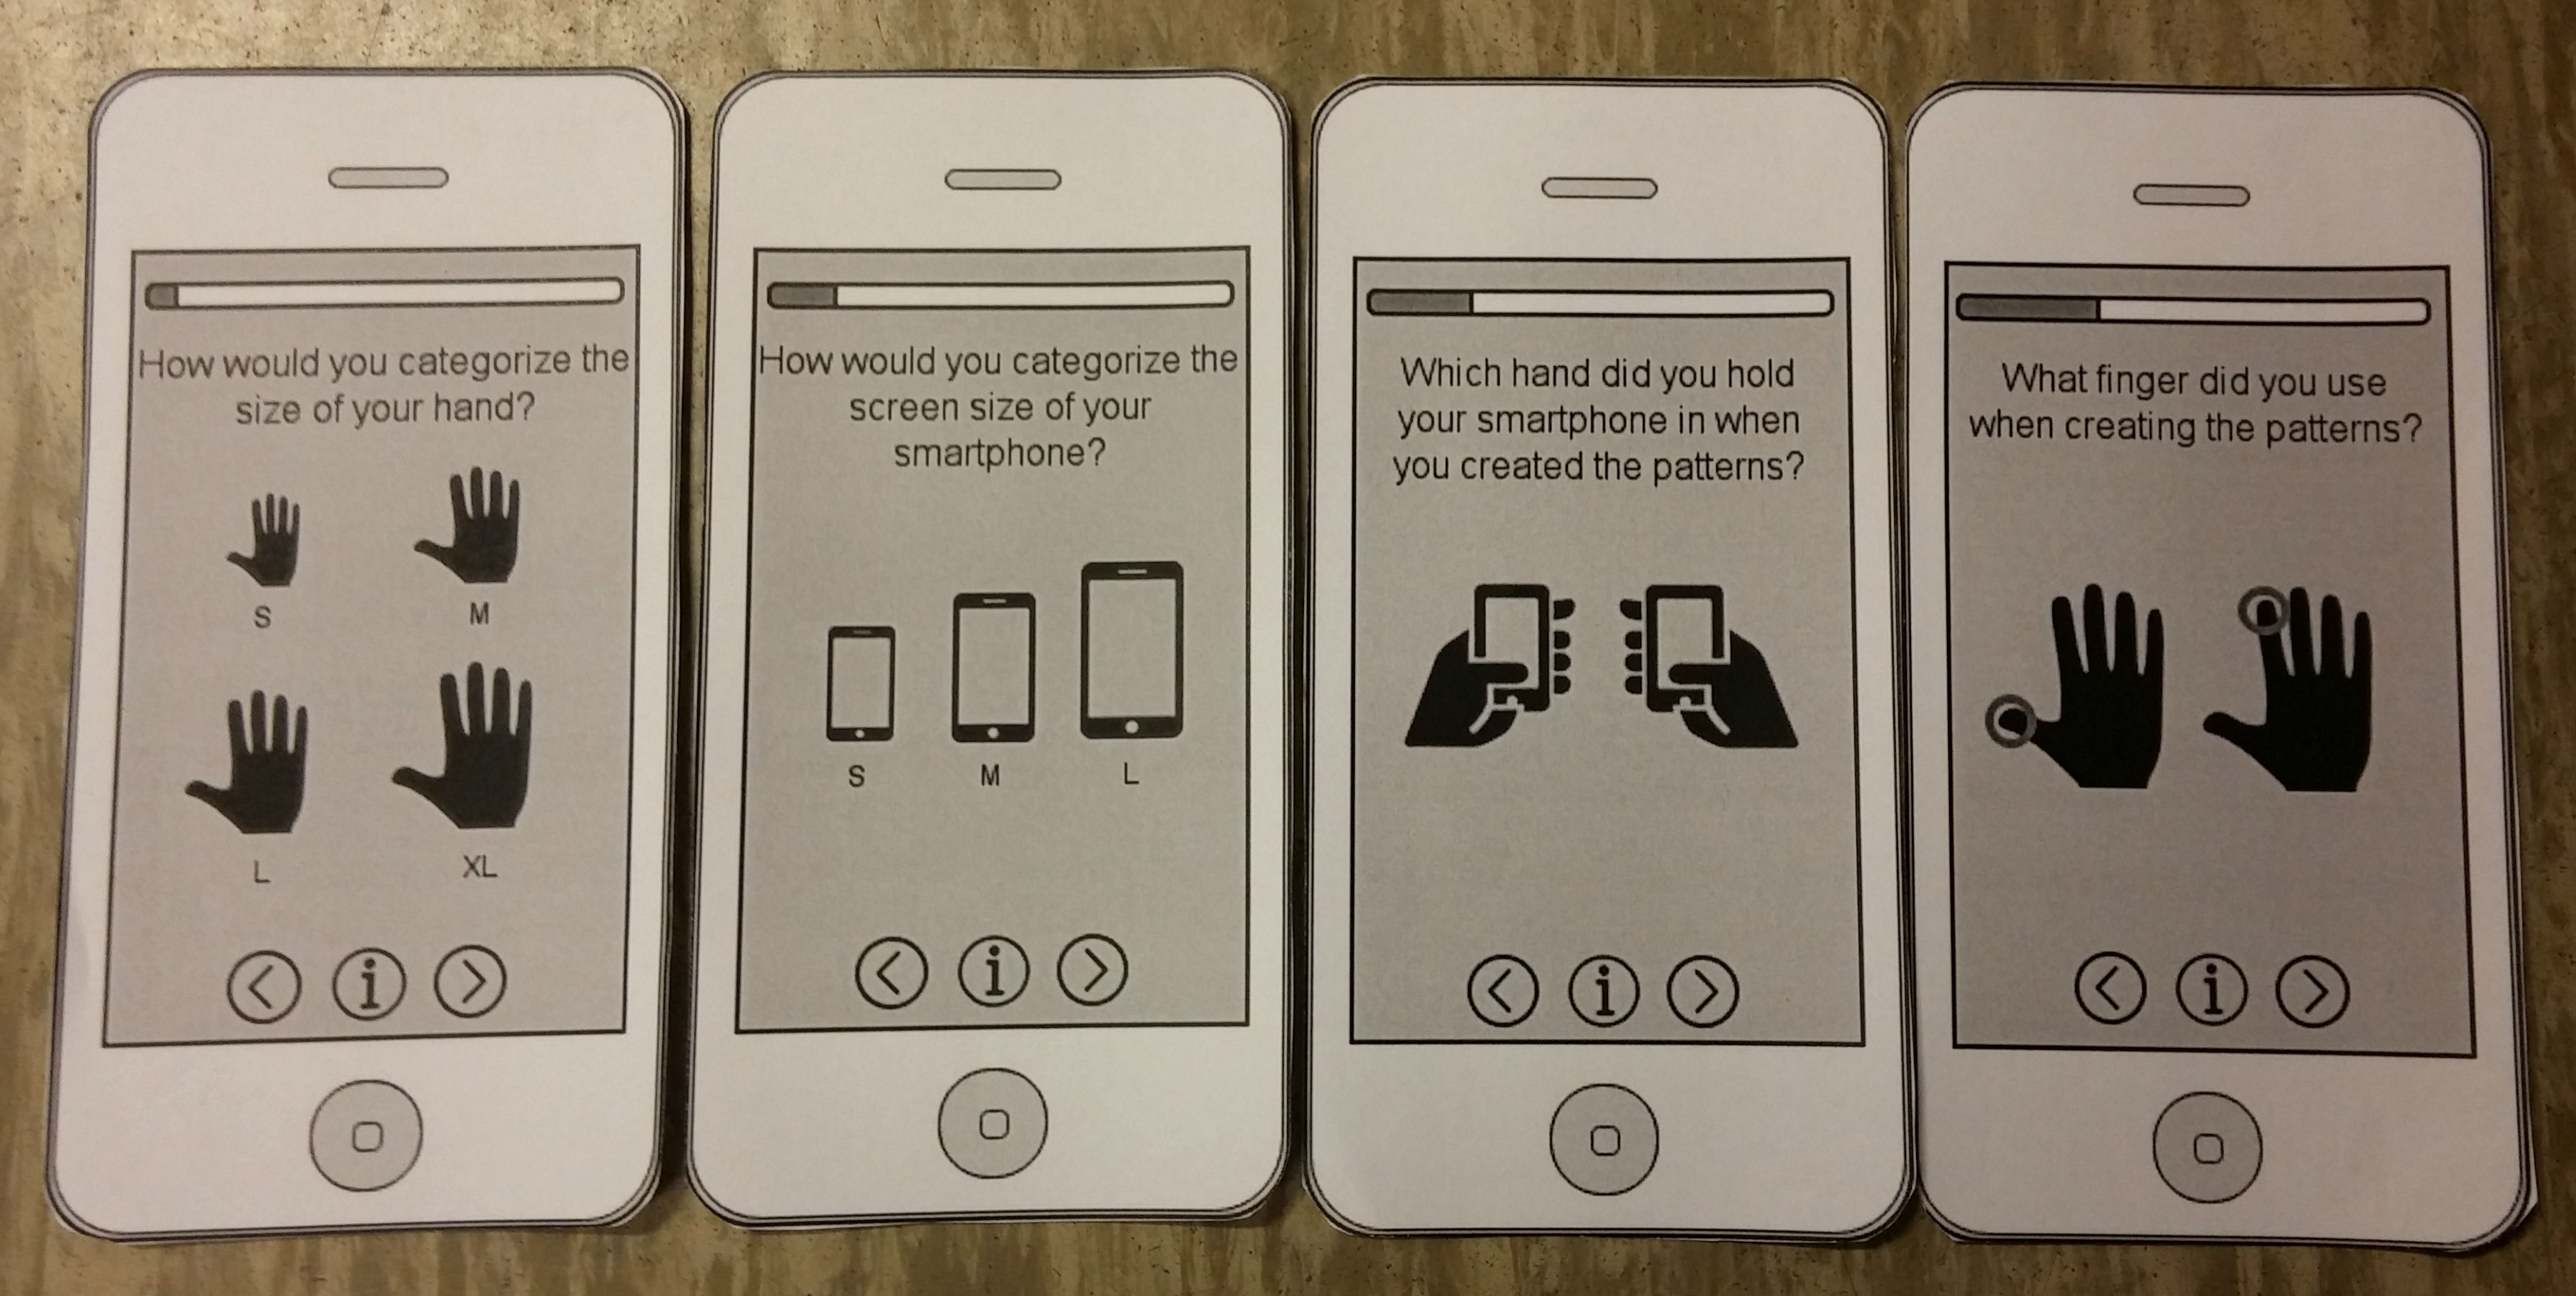
\includegraphics[width=\textwidth]{pics/test1.png}
      \caption{Usability test 1}
      \label{fig:test1}
    \end{figure}

  In the second test, it only tested the effectiveness (measured in number of errors) by only looking at the icons. When showing the icons to the participant, the actual question was covered. The students that participated in the test was supposed to guess what was asked for and select their answer by only looking at the icons. When conducting this test, the goal was to be able to see if the icons was understandable. When sending out the questionnaire, it is important that respondent that are not fluent in English are able to answer the questions without be able to understand all the English words. It is also useful for respondents to be able to use the text and the icons together in order to understand the questions. Figure~\ref{fig:test2} is showing an image from test 2, where the question is covered. 

    \begin{figure}[H]
      \centering
      \includegraphics[scale=0.2]{pics/test2.png}
      \caption{Usability test 2}
      \label{fig:test2}
    \end{figure}

  \subsubsection*{Results}

  For testing the prototype, I contacted five girls and five boys (age from 20-24) from the university, resulting in 5 participants in each test. This is a small number of participants and does only represent a small part of the population. The primary goal was to get some feedback on the wireframes from Section~\ref{fig:wireframes}. The participants were explained that the test did not test their knowledge, rather the systems and its design. If they ever felt uncomfortable, they were also told that they could quit the test whenever they wanted. The feedback from the participants will be included in the next version of the prototype. The new prototype will be tested and implemented next semester.

  In test 1, all the wireframes were used and was demonstrated in the same order as Figure~\ref{fig:wireframes}. Before they started on the questionnaire, they were given information about the research, their right to stay anonymous, and the purpose of the research. The participants began when they pressed ``Start'' as illustrated in Figure~\ref{fig:wireframe1}. During the test, the participants commented on some part of the test.

  {\bf Comment on Figure~\ref{fig:wireframe20}}: {\it "I study, but I have not finished my studies. Should I press yes?"}. All of the respondents was unsure whether to select "yes" or "no" in order to answer the question about their experience with IT and security. All the participants were IT-students, and all was unsure if the word ``studied'' was fitting their situation since they still were students. Most of the students chose to select ``no'' as their answers, but I would probably categorize all of them in a group experienced with IT and/or security. This question should be rephrased in order to avoid respondents to get in the same position.

  {\bf Comment on Figure~\ref{fig:wireframe12}}: {\it "What do you mean by reading and writing orientation?"}. One of the students were unsure what the question asked. The student guessed that the question posed for the direction that he used to write, but he got unsure when he read the ``top-to-bottom'' alternative because he could not relate to the alternative. He then clicked on the information button, and I explained what the different reading orientation was.

  {\bf Comment on the progress bar}: The progress bar in the prototype is very simple, and do not indicate how many questions that is left. Only one participant commented on this. He would like to see exactly how many questions that was answered and how many questions that is left. He suggested that he it could be used dots that are often used together with swipe navigation. He also added that this probably would be hard to implement because of the number of questions. An alternative suggestion was to remove the information icon next to the question and replace it with the number of questions answers (for example 2/12, two out of twelve questions answered).

  {\bf Comment about the pattern creation}: {\it "I would like to create a pattern for the smartphone first because I wanted to use the pattern from my own smartphone because that is something I am familiar with"}.

  After the participants had completed the questions, I asked a set of predefined questions:

  {\bf Question 1 - Navigation}: All the participants were asked how they felt about the flow and navigation in the system. The reason this question is asked is because the prototype has two arrows that are indicating how to get to the next question. On mobile devices, it is desirable to have the least possible amount of clicks in order to use less time. Pressing the same button to go to the next question can for some users be annoying. The arrows are added to the prototype because it is hard to simulate automatic animation or swipe navigation on paper. The participants got a chance to express how they would like the navigation to be, and how they would expect it to work. All the respondents would like the questions to navigate automatically when they selected their answers. Some of the participants commented that they wanted the icons to change color, and then see an animation of the automatic animation. Some of the participants that wanted the automatic navigation added the comment that they wanted to be able to go back if they chose the wrong answer. So if the automatic navigation was added, then there was a need to be able to go back, so they did not lose control. Two of the respondents wanted the questionnaire to support swipe navigation because they expect that this is how website navigation works.

  {\bf Question 2 - Trustworthiness}: All the respondents were asked if they felt confident when they answered the questionnaire. Asking people to give away patterns might result in loosing some respondents because they do not feel confident. It is, therefore, important to provide enough information about the research and how the data is going to be used. The trustworthiness is important to obtain from the respondents already in the introduction.

  In test 2, the respondents were challenged with the wireframes that contained icons. They guessed what was asked for and then selected they answer with an explanation of why they did so. All the five respondents (three girls and two boys) managed to interpret the icons and guess most of the questions. There was one participant that guessed that the wireframe in Figure~\ref{fig:wireframe16} was asking if they used the Android scheme. It is quite close, but not the exact question. I do not see this as a problem because all the respondents from test 1 manage to interpret the question correctly. One drawback with this test is that the icons are quite simple, and some of them might not be good enough for the actual implementation.

  The results of both tests are providing valuable information that will be used to make suggestions for redesign. The Suggested improvements are further described as suggestions in the chapter for further work.
  
	\section{Ethical Consierations}


	% Chapter 5 - Further Work
	\chapter{Further Work}

	%Bibtex
	\bibliographystyle{plain}
	\bibliography{myBib}
	
	\todo{Renskrive of sjekke kilder!}

\end{document}